% !TEX TS-program = pdflatex
% !TEX encoding = UTF-8 Unicode

\documentclass[a4paper, oneside, justified=true, sfsidenotes]{tufte-book} 
\usepackage[utf8]{inputenc} % set input encoding to utf8
\usepackage[greek, french,english]{babel}[2005/11/23]
\usepackage{lipsum}
\usepackage{listings}
\usepackage{lineno}
\usepackage{xcolor}
\usepackage{gantt}
\usepackage{booktabs}
\usepackage{goodlists}
%% Bibliography
\usepackage{natbib}

\bibliographystyle{plainnat} % note the change here
\bibpunct{(}{)}{;}{a}{,}{,}


\usepackage{amsmath}[2000/07/18] %% Displayed equations
\usepackage{amssymb}[2002/01/22] %% and additional symbols

\usepackage{alltt}[1997/06/16]   %% boilerplate, credits, license
\usepackage{epigraph}
\usepackage{graphicx}

\usepackage{caption}
\DeclareCaptionFont{blue}{\color{blue}}
\captionsetup{justification=raggedright, singlelinecheck=false,font={blue,sf,small}}

\usepgflibrary{shapes.symbols}
\usetikzlibrary{positioning, shapes, arrows, chains}
\usepackage{pgfplots}
\usepackage{comment}
%overwrite tufte and have numbering
\setcounter{secnumdepth}{5}


%% Change some of the looks
%%% CHAPTER STYLES AND SECTION STYLES
\pagestyle{fancy}
\renewcommand{\chaptermark}[1]%
{\markboth{\MakeUppercase{\chaptertitlename\ \thechapter\ #1}}{}} %no dot here
\renewcommand{\sectionmark}[1]%
{\markright{\MakeUppercase{\thesection~\ #1}}}
\renewcommand{\headrulewidth}{0.5pt}
\renewcommand{\footrulewidth}{0pt}
\newcommand{\helv}{%
\fontfamily{phv}\fontseries{b}\fontsize{9}{11}\selectfont}
\fancyhf{}
\fancyhead[LE,RO]{\helv \thepage}
\fancyhead[LO]{\helv \rightmark}
\fancyhead[RE]{\helv \leftmark}

%%hyperref
\hypersetup{urlcolor=green, colorlinks=true}  % Colours hyperlinks in blue, but this can be distracting if there are many links
\urlstyle{sf}  %set url as sans-serif font (in url? find how to do with hyperref)





% Typesets the font size, leading, and measure in the form of 10/12x26 pc.
\newcommand{\measure}[3]{#1/#2$\times$\unit[#3]{pc}}

% Macros for typesetting the documentation

\newcommand{\fox}{\medskip  "The quick brown fox jumps over the lazy dog"\medskip} % mini lorem
\newcommand{\dogs}{The sentence is often mistakenly rendered as "The quick brown fox jumped over the lazy dog," which does not include an s. However, this can be corrected by typing: "The quick brown fox jumped over the lazy dogs".}


\newcommand{\hlred}[1]{\textcolor{Maroon}{#1}}% prints in red

\newcommand{\hlmaroon}[1]{\textcolor{Maroon}{#1}}%print maroon

\newcommand{\hangleft}[1]{\makebox[0pt][r]{#1}}


\newcommand{\sourceatright}[2]{{%
  \unskip\nobreak\hfil\penalty100
  \hskip#1\hbox{}\nobreak\hfil{#2}
  \parfillskip 15pt \par}}


\newcommand{\hairsp}{\hspace{1pt}}% hair space
\newcommand{\hquad}{\hskip0.5em\relax}% half quad space
\newcommand{\TODO}{\textcolor{red}{\bf TODO!}\xspace}

\newcommand{\ie}{\textit{i.\hairsp{}e.}\xspace}
\newcommand{\eg}{\textit{e.\hairsp{}g.}\xspace}


%\newcommand{\na}{\quad--}% used in tables for N/A cells

\providecommand{\XeLaTeX}{X\lower.5ex\hbox{\kern-0.15em\reflectbox{E}}\kern-0.1em\LaTeX}
\newcommand{\tXeLaTeX}{\XeLaTeX\index{XeLaTeX@\protect\XeLaTeX}}
% \index{\texttt{\textbackslash xyz}@\hangleft{\texttt{\textbackslash}}\texttt{xyz}}

%% define backsalsh
%% you can also use \textbackslash
\newcommand{\tuftebs}{\symbol{'134}}% a backslash in tt type in OT1/T1

\newcommand{\doccmdnoindex}[2][]{\texttt{\tuftebs#2}}% command name -- adds backslash automatically (and doesn't add cmd to the index)

\newcommand{\doccmddef}[2][]{%
  \hlred{\texttt{\tuftebs#2}}\label{cmd:#2}%
  \ifthenelse{\isempty{#1}}%
    {% add the command to the index
      \index{#2 command@\protect\hangleft{\texttt{\tuftebs}}\texttt{#2}}% command name
    }%
    {% add the command and package to the index
      \index{#2 command@\protect\hangleft{\texttt{\tuftebs}}\texttt{#2} (\texttt{#1} package)}% command name
      \index{#1 package@\texttt{#1} package}\index{packages!#1@\texttt{#1}}% package name
    }%
}% command name -- adds backslash automatically

%% doc commands
% % adds hem automatically to index

\newcommand{\doccmd}[2][]{%
  \texttt{\hlred{\tuftebs#2}}%
    \ifthenelse{\isempty{#1}}%
    {% add the command to the index
      \index{#2 command@\protect\hangleft{\texttt{\tuftebs}}\texttt{#2}}% command name
      % \marginpar{\hlred{#1}}
    }%
    {% add the command and package to the index
      \index{#2 command@\protect\hangleft{\texttt{\tuftebs}}\texttt{#2} (\texttt{#1} package)}% command name
     \index{#1 package@\texttt{#1} package}\index{packages!#1@\texttt{#1}}% package name
    }%
}% command name -- adds backslash automatically



%% doc options
%
\newcommand{\docopt}[1]{\ensuremath{\langle}\textrm{\textit{#1}}\ensuremath{\rangle}}% optional command argument


\newcommand{\docarg}[1]{\textrm{\textit{#1}}}% (required) command argument
\newenvironment{docspec}{\begin{quotation}\ttfamily\parskip0pt\parindent0pt\ignorespaces}{\end{quotation}}% command specification environment


\newcommand{\docenv}[1]{\texttt{#1}\index{#1 environment@\texttt{#1} environment}\index{environments!#1@\texttt{#1}}}% environment name


\newcommand{\docenvdef}[1]{\hlred{\texttt{#1}}\label{env:#1}\index{#1 environment@\texttt{#1} environment}\index{environments!#1@\texttt{#1}}}% environment name

%% Provide a  command to add packages to index
%
\newcommand{\docpkg}[1]{\hlred{\texttt{#1}}\index{#1 package@\texttt{#1} package}\index{packages!#1@\texttt{#1}}
\marginpar{\hlred{#1~package}}
}% package name

%% Provide a command for document cls - do not add to index
%
\newcommand{\doccls}[1]{\texttt{#1}}% document class name


\newcommand{\docclsopt}[1]{\texttt{#1}\index{#1 class option@\texttt{#1} class option}\index{class options!#1@\texttt{#1}}}% document class option name
\newcommand{\docclsoptdef}[1]{\hlred{\texttt{#1}}\label{clsopt:#1}\index{#1 class option@\texttt{#1} class option}\index{class options!#1@\texttt{#1}}}% document class option name defined
\newcommand{\docmsg}[2]{\bigskip\begin{fullwidth}\noindent\ttfamily#1\end{fullwidth}\medskip\par\noindent#2}
\newcommand{\docfilehook}[2]{\texttt{#1}\index{file hooks!#2}\index{#1@\texttt{#1}}}
\newcommand{\doccounter}[1]{\texttt{#1}\index{#1 counter@\texttt{#1} counter}}

%% margin document commands
%
\newcommand{\margindoc}[1]{\marginpar[]{\doccmd{#1}}}

\newcommand{\sidebarcolor}[1]{\textcolor{darkgray}{\sidenote[]{#1}}}

%% alias of \doccmnd
\newcommand{\cmd}[1]{\doccmd{#1} \marginpar[]{\hlred{\doccmd{#1}}}}


%% Set up the epigraph to be a bit wider
\setlength{\epigraphwidth}{8cm} 
\setlength{\epigraphrule}{0pt}
\newcommand{\theepigraph}[2]{\epigraphhead[30]{\epigraph{#1}{\textit{#2}}}}




\newcommand{\bs}{$backslash$}



\title{CONSTRUCTION \\ MANUAL FOR MEP}
\author{City Center Phase 3a \&3b}
\publisher{AL HABTOOR-Specon}
\date{January 2011} % Delete this line to display the current date
\usepackage{float}
\usepackage{wrapfig}

% Generates the index we use before the
% out
\usepackage{makeidx}
\makeindex





\usepackage{amsmath}
\usepackage{amsfonts}
\usepackage{amssymb}[2002/01/22] %% and additional symbols



\usepackage{longtable}



%% Set some local commands and colors
\usepackage{colortbl}
\definecolor{green}{rgb}{0.1,0.1,0.1}
%\color{green!40!yellow})

\newcommand{\done}{\cellcolor{teal}done}  %{0.9}
\newcommand{\hcyan}[1]{{\color{teal} #1}}

%% Use the graphics package
% For graphics / images
\usepackage{graphicx}
\setkeys{Gin}{width=\linewidth,totalheight=\textheight,keepaspectratio}
\graphicspath{{graphics/}}


\usepackage[pages=some,placement=top]{background}

\usepackage{soul}

%% hack not to leave blank pages before chapters
%%


\makeatletter
\def\chapter{\clearpage\thispagestyle{plain}\global\@topnum
  \z@\@afterindentfalse
  \secdef\@chapter\@schapter
}
\makeatother


\definecolor{activity1}{rgb}{0,1.0,0}
\definecolor{activity2}{rgb}{0,0.9,0}
\definecolor{activity3}{rgb}{0,0.85,0}
\definecolor{activity4}{rgb}{0,0.75,0}
\definecolor{activity5}{rgb}{0,0.65,0}


%% Color helper routine
\def\getcolor#1#2{%
\def\zero{0}\def\one{1}\def\two{2}%
\if\zero#1 \gdef\statuscolor{white} \else \gdef\statuscolor{#2}\fi%
\if\two#1  \gdef\statuscolor{red} \fi%
}

\gdef\ascale{0.8}

\gdef\floor#1#2#3#4#5#6{%
\centering%
\parindent0pt%
\tikzpicture[scale=\ascale]%
\def\posx{0.6}%
\getcolor{#2}{activity1}%
\draw node [anchor=south east]{#1}; % places label
\draw[fill=\statuscolor] (0,0) rectangle (0.5,0.5); 
\getcolor{#3}{activity2}
\draw[fill=\statuscolor] (\posx,0.0) rectangle (1.1,0.5);
\getcolor{#4}{activity3}
\draw[fill=\statuscolor] (2*\posx,0.0) rectangle (1.7,0.5);
\getcolor{#5}{activity4}
\draw[fill=\statuscolor] (3*\posx,0.0) rectangle (2.3,0.5);
\getcolor{#6}{activity5}
\draw[fill=\statuscolor] (4*\posx,0.0) rectangle (2.9,0.5);
\endtikzpicture%
}

% counter used in tables
\newcounter{inc}
\def\inc{\addtocounter{inc}{1}\theinc}

\begin{document}

\newcommand{\project}{City Center Phase 3a \& 3b}
\newcommand{\msnumber}{MS-HS-118-MC-005}
\newcommand{\client}{Al-Rayyan Tourism Industry Company}
\newcommand{\consultant}{HOK, MSCEB}
\newcommand{\projectmanager}{CANSULT}
\newcommand{\maincontractor}{Al Habtoor Engineering}
\newcommand{\msname}{Method Statement for the Commissioning of Chilled Water Pumps}
\newcommand{\maincontractorshort}{HEE} % main Contrator initials
\newcommand{\consultantshort}{EHAF} % Consultant initials
\newcommand{\projectname}{\Large {City Center Phase 3a \& 3b}}

\newcommand{\signatureblock}{
\begin{tabular}{|l|l|l|l|}
\noalign{}\hline
 CONTRACTOR APPROVAL                &                &                     & \\
\noalign{}\hline
SPECON    & NAME~~~~~~~~~~~     & SIGNATURE~~~~~~~~~~  & DATE~~~~~~~~~~~~\\
\noalign{}\hline\hline
\noalign{}\hline
 CONSULTANT APPROVAL                &                &                     & \\
\noalign{}\hline
EHAF    & NAME~~~~~~~~~~~     & SIGNATURE~~~~~~~~~~~~~~~  & DATE \\
\noalign{}\hline
\end{tabular}
}

% checkboxes
\newcommand{\checkboxes}{
Yes~No {\Large ~$\Box$}~~~ {\Large $\Box$}
}

% Common Definitions for alll Method Statements

%1	Wild Air Methodology	Specon
%2	Commissioning Methodology and Organization	Specon
%3	CHW System Flushing & Chemical Treatment	Specon
%4	Air & CHW Balancing	TAB Agency
%5	Chilled Water Pump	Specon/Supplier
%6	Plate Heat Exchangers	Specon/Supplier
%7	Boiler Package	Specon/Supplier
%8	Cooling Towers	Specon/supplier
%9	Pressurisation Unit	Specon/Supplier
%10	Ecological Units	Specon/Supplier
%11	Building Automation System(FCU's Test Pack)	Specon
%12	Domestic Water Filtration -System Operation	Specon/Supplier
%13	Condenser Water System(Cold Rooms)	Specon
%14	Smoke Extract System(Carpark)	Specon/Supplier
%15	Kitchen Extract System	Specon
%16	Staircase pressurisation	Specon
%17	Kitchen Exhaust Smoke Test	Specon
%18	CO Monitoring & Clearance(Inc Cause&Effect)	Specon/Supplier
%19	Building Management System	Specon/Supplier

%Hydraulic Services		
%20	Plumbing Pumps	Specon
%21	Chlorination	Specon/Supplier
%22	Grey Water & Flush Water System	Specon/Supplier
%23	Domestic Water - System Operation	Specon
%24	Domestic Hot Water - System Operation	Specon
%25	Condenser Water Treatment	Specon
%26	Drainage System	Specon
%27	LTHW Water Treatment	Specon/Supplier
%28	Irrigation System	Specon/Supplier

%Fire Services		
%29	Sprinkler Hose Reel & Fire Hydrant System	Specon/Naffco
%30	Fire Pumps/Fire Panels	Specon/Naffco
%31	FM 200 System	Specon/Naffco
%32	Heliport Fire Protection Testing & Comm.Procedure	Specon/Naffco

% Gas Services		
%33	LPG	Specon/Gaspro
		
%Electrical Services		
%39	Transformer	Specon/Supplier
%40	MV Panels	Specon/Supplier
%41	SMDB	Specon/Supplier
%42	Distribution Boards & Sub Circuits	Specon
%43	Room & Apartment DB & Sub Circuits	Specon
%44	Power Factor Capacitor Banks	Specon/Supplier
%45	MCP/VSD/ATS	Specon/Supplier
%46	MCC Panels	Specon/Supplier
%47	AMF Panels (DG)	Specon/Supplier
%48	DG Auxiliary Panels	Specon/Supplier
%49	Generator System	Specon/Supplier
%50	UPS System	Specon/Supplier
%51	Earthing System	Specon
%52	Feeder Cables	Specon
%53	EMERGENCY Lighting Functional Test	Specon/Supplier
%54	Lightning Protection System	Specon/Supplier
%55	Heliport Lighting System	Specon/Supplier
%56	Aircraft Warning Light System	Specon/Supplier

%Electrical ELV Systems		
%57	Dimming System	Specon
%58	Façade Lighting	Specon
%59	Intrusion Alarm System	Specon/Supplier
%60	CCTV System	Specon/Supplier
%61	Car Calling System	Specon/Supplier
%62	Telephone & Data System	Specon/Supplier
%63	IPTV System	Specon/Supplier
%64	Intercom System	Specon/Suppler
%65	Two Way Radio System	Specon/Supplier
%66	Audio Visual & Back Ground Music System	Specon/Supplier
%38	Fire Alarm System	Specon/supplier

\newcommand{\msnumberstring}{MS-HS-118-C-001}

\newcommand{\hotels}{the Rotana and Shangrila hotels }












\SetBgContents{Update $13^{th}$ Jan 2013}
\BgThispage
% Front matter
\frontmatter

% r.1 blank page
%\blankpage


% r.3 full title page



% r.5 contents
\maketitle
\tableofcontents
\listoffigures
\listoftables

\chapter{Document Control}

\section*{What problem are we trying to solve?}
\begin{marginfigure}
  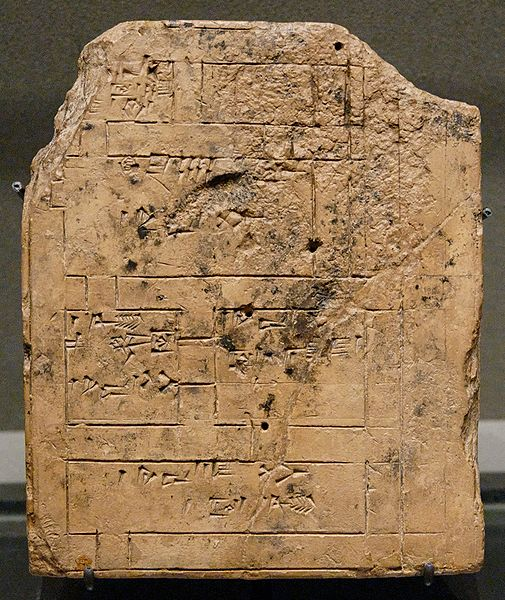
\includegraphics[width=\linewidth]{gudea-plans}
  \caption{Clay plans of a six-room building, a sanctuary or a private house. From Telloh, ancient Girsu circa 2125, from \url{http://en.wikipedia.org/wiki/Gudea_cylinders}}
  \label{fig:marginfig1}
\end{marginfigure}
If you ever lost a document you will agree that there is always a need to keep control of important documents. The document control system has been designed to aid in the  filing of documents and provide an easy way of retrieving this information.
Some documents we keep because is required by law to keep them. Others we need them in order to control the flow of money in a Company. To summarize the system described in this chapter will help you file your documents better and enable you to retrieve these documents easier.

\section*{What is document control?}

Document control means that the right persons have the current version of the documents they need, while unauthorized persons are prevented access to them.

We all handle many documents every day. These documents include forms that we fill out, instructions that we follow, invoices that we enter into the computer system, holiday schedules that we check for the next day off, rate sheet that we use to bill out customers, and many more.

An error on any of these documents could lead to problems. Using an outdated version could lead to problems. Not knowing if we have the latest version or not could lead to problems. And so on.

The Document control system affects our entire company, and all business related documents must be controlled. Only documents that don’t have an impact on our products, services or company don’t need to be controlled – all others need to be controlled. This means, basically, that any business related documents must be controlled. 

\section*{Whose responsibility?}

\begin{marginfigure}
  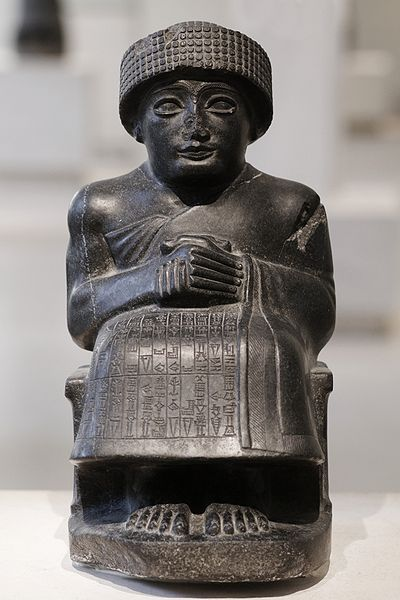
\includegraphics[width=\linewidth]{gudea}
  \caption{Diorite statue od the earliest known document Controller. Mesopotamia circa 2150 BC.}
  \label{fig:marginfig1}
\end{marginfigure}

Document control is the responsibility of all employees. It is important that all employees understand the purpose of document control and the tools (requirements) that help us control our documents.

Please be aware that if you copy a document or print one out and then distribute it, you are responsible for controlling the distribution! The original author won't know that you distributed more of his documents, so the original author can't control that distribution. That is why on critical job sites all copies, faxing and distribution is via our DCC (Document Control Center)






\section*{Project Filing}

%\begin{marginfigure}
%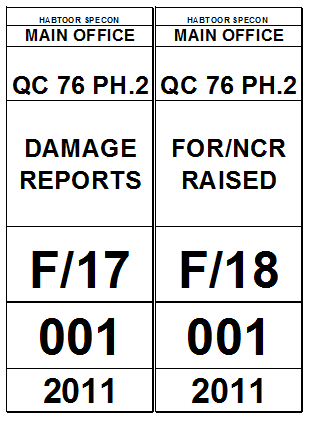
\includegraphics[width=\linewidth]{labels}
%\caption{Filing labels}
%\end{marginfigure}

\begin{marginfigure}
  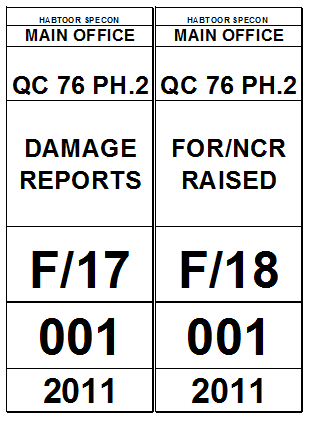
\includegraphics[width=\linewidth]{labels}
  \caption{Calorifier plant-room in Merweb.}
  \label{fig:marginfig1}
\end{marginfigure}

Project filing, follows closely to the system set up at Head Office. You can think of Document Control a bit like the post office where communication is always between one office to another. In many respects filing on sites is more difficult and challenging due to its temporary nature and the changing number of employees as the Project moves through the different phases.

Files are labeled with letters and numbers:

\begin{center}
\fbox{
       \begin{minipage}{6.0cm}
        FILE REF. NO. A/1

        Outgoing Correspondence.
       \end{minipage}
}
\end{center}
        
When files overflow we number them consequentially as follows:

\begin{center}
\fbox{
       \begin{minipage}{6.0cm}
        FILE REF. NO. A/1-001

        Outgoing Correspondence.

        FILE REF. NO. A/1-002

        Outgoing Correspondence.
 \end{minipage}
}
\end{center}

The file references are initially chosen to represent a comprehensive Master File list. An extract from such a Master List is in Table\ref{masterlist}.


\begin{fullwidth}
\begin{table}[htb]
\vspace{0.5cm}

\small
\hskip-10pt\begin{tabular}{|l|l|l|l||l|l||l|l||l|l|l|}
\hline
File &Category        &Control              & Person       &Copy 1  &Person        &Copy 2        &Person      &Copy 3 &Person\\
     &                &Copy location        & resp. &        &resp.   &resp.   &resp. &      &resp.\\
\hline
A/1    & Corresp (in).       & H.O. Sec.           & H.O. Secr. & Site & PM           &              &            &      & \\
A/2    & Corresp.(out)       & H.O. Sec.           & H.O. Secr. & Site & PM           &              &            &      & \\
A/3    & memos (in)          & H.O. Sec.           & H.O. Secr. & Site & PM           &              &            &      & \\
A/4    & memos (out)         & H.O. Sec.           & H.O. Secr. & Site & PM           &              &            &      & \\
\hline
\end{tabular} 	
\caption{Extract from filing list}
\label{masterlist}
\end{table}
\end{fullwidth}

What is important to notice in the Table above, that in many cases the filing system allows for up to three copies to be kept, but there is always a two tier system where there is a \textit{control copy}, normally kept at head office and one or two copies kept at other locations. If the site is far from head office or for cases where there is no need to keep copies at Head Office the Document Control Department always keeps the master copy.

It is also important to note that documents have \textit{owners}. In the extract shown in Table\ref{masterlist}. The owner is the responsible person to make sure that the documents have been filed properly. In most cases this person in the Project Document Controller, but for example for orders the Materials Control Manager is the ultimate responsible person to ensure that MCD documents are filed properly.

\subsection*{Document Order}

In general document are filed by \textit{date order}. Numbered documents such as submittals, Quality Assurance Documents and the like bear that bear \textit{reference numbers} are filed \textit{sequentially}. Accounting documents
such as creditors invoices are filed by \textit{date} in the master file and a second copy by \textit{Creditors name}. By choosing
carefully the method of filing and normally by having two different methods enables retrieval of the document easier. In general if the system
is computerized retrieval becomes easier.  

\section*{Setting up the system}

The filing system should be set at the begining of a new Project. Although this sounds simple and intuitive most Projects start without adequate
space, building shelving as we go and continuously buying files. On a well designed system \textit{all} file categories are set up when the Project starts, they are labelled uniformly. As a rule of thumb the minimum space is that of a 20 foot container - and this assuming that files with multiple volumes are archived at certain points. If you do not give it attention at the beginning of the Project you will literally
drawn in paper work nobody will be able to find anything and  everyone will build their own system as they will not have any \textit{faith} in yours!

The equation below, can be used to estimate the number of files that will be required for a project:



$$ N = \frac{p^{0.8}(t + d)}{d} $$

where,

N = number of files

p = mean personnel on project

t = duration of project (months)

d = number of departments




\section*{When to file}

Generally if people responsible for filing do not clear their intrays daily it leads to problems with retrieval. What happens as they have a continuous backlog the bottom of the tray never gets cleared and after a week or two documents cannot be found (so we get another copy from whoever sent it to us) which leads to another problem that eventually when we find the document we now have two identical copies in the file and 
stamped with two different incoming date stamps.

\section*{Getting the right equipment}

During the two critical \textit{crunch periods} of the Project, which are normally the start and end of the Project you will find that
documents and document copying and processing is at its peak. During this time of the project unless the Site and its partner Companies have a decent photocopier the flow of documents will slow down tremendously. It is not unknown for documents to take 11 days to be delivered from the Consultant's desk (via their own document control) to that of the Main contractors's and then to us. For comparison in 1890 a letter would travel at the cost of 1 penny with the Imperial Penny Post from London to Cape Town by steam ship in less than 20 days and taht was door to door delivery. In general a decent photocopier should be purchased based on expected volumes of copying which should never be less than 20000 copies per month (to keep up with peaks). This should be able to interface with a computer and the network and if you are going to charge subcontractors  departments or Clients it should have a keypad for logging usage. When the latter is not used, it is also not unknown for people to introduce 
manual systems of approval and logging of copies usage introducing another cost to the Company and further contributing to bureacratic bloat, inefficiency and delays. 

\section*{Key performance indicators}

Document Control should be able to produce all necessary log forms weekly by close of business every Thursday or at a date agreed with the Project Director. Normally these are:

\begin{table}
\begin{tabular}{l}
\toprule
Material Submittal logs\\
RFI logs\\
WIR logs\\
\bottomrule
\end{tabular}
\caption{Weekly logs produced by Document Control}
\end{table}


Document Control should be able to retrieve a document within a maximum of 30 minutes and deliver a copy (right? you don't want the original copies to leave Document Control - so you do need a good and fast photocopier). The best performance indicator is for the Document Control Department is to keep it \textit{customers} happy. 

\section*{Dating documents}

Require us to show on every document when it was created or last updated. Many of us thought about using the automatic date field for this but….
Should we use the automatic date field on documents?

Generally not, if you enter the automatic date field into a document, the field will automatically be updated to always show the current date, no matter when you actually created or updated the document.



Another example:

Another example is entering the automatic date field in the footer of a document that you frequently change and then print. You may have used the automatic date field as an easy way to see on your printouts when they were printed; the idea here was that the document with the latest date is the most current printout. However, you may make one printout today and another tomorrow without having made any changes to the document. Though both printouts are identical, they now show different dates. This will inevitably lead to confusion. 

Document control requires us to show on any document when it was created or last updated. The automatic date field is not suitable for this. Therefore, as a general rule, don’t use the automatic date field to identify version status.


\section*{Forms}

Yes, a form must be controlled as long as the form has an impact on our services or our company.

Blank forms are similar to instructions as they guide the user to provide certain information. If the form is outdated or incomplete, the user will not be prompted to supply all the necessary information. It is, therefore, important to control blank forms like any other document.

Once a form is filled out, however, it has become a record. At this point, we need to be concerned with filing, storage, archiving, and eventually destruction.
All forms and documents are specified in the Company ISO Manual.

\section*{Policies and procedures}

While most procedure affect only managers, all employee must be familiar with the \textit{Quality Policy} and with the \textit{Document Control Procedure}.

\section*{Document Control Organization}

The Document control department is actually a Main Department and sattelites. Sattelite sections will exist in other Departments. In general it should be organized as follows:

\begin{verbatim}
- Document Control (Central Department)
-- Administration /HR (visa related, personnel passports, drivers, petrol control)
-- Correspondence (secretary)
-- QA/QC
-- QS
-- Procurement
-- Design (very limited)
-- CAD Office
-- Accounts
-- Stores (own copies of delivery notes, returns issues etc).
-- Safety department
\end{verbatim}

The particular contributions of these departments are laid out in their respective Business process sections. The Document Control department is normally staffed with 3-4 people. The Document Controller, one or two assistants and a person dedicated to photo-copying. 


\section*{Computerized Systems}

Computerized systems do not eliminate the need for paper filing but can reduce it. They can also assist in retrieval and distribution. Unless
your manual system is working well, computerization is next to impossible.


\section*{Archiving and disposal of documents}
\begin{marginfigure}
  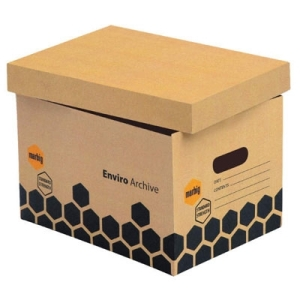
\includegraphics[width=\linewidth]{archivebox}
  \caption{Environmental friendly box}
  \label{fig:marginfig1}
\end{marginfigure}
At the end of the Project most of the items will require to be disposed or archived. Having now contributed considerably to the destruction of the environment by using all this paper and possibly finished a monstrosity on a pristine location, this can be done by buying environmentally friendly boxes made for the purpose. Documents to be disposed should be shredded if possible. If the system has been followed and monitored, this should be a simple operation as all the filing will already be in boxes and what it means is that only the last files will be boxed. Label the boxes accordingly and state the date that the contents can be disposed off.

\section*{Summary}

This short document described some of the issues relating to the control of Company documents. As a last word do some kaizen.\sidenote{\href{Kaizen}{http://en.wikipedia.org/wiki/Kaizen}.}






























\chapter{Materials Control Department}

\begin{quotation}
 If you're buying a product then you need to spend money to hire sophisticated buyers, because if your buyers are dumber than the sales-people you're buying from they're going to be fleeced.
\end{quotation}

The Materials Control Department on a Project is the responsible department that ensures that materials are purchased at the \textit{least possible price, they
meet the Project quality standards  and that they are delivered on time}. 

\section*{Materials Planning}
This is the most difficult phase of teh procurement cycle and if not planned
properly the MCD department will be in \textit{panic mode} until the end of the
Project. At the beginning of the Project a Materials Control Sheet is created
listing all the material requirements of the Project by categories. Categories
are normally split in such a way that a category is materials purchased from a single
vendor.

At the beginning of the Project at the discretion of the Area Manager and the Project
Director, the Engineering Office as well as all the Engineers and perhaps the
CAD Office will contribute to material take-offs. The Engineering Office
will also handle enquiries and discussions with Suppliers for items where
a strong technical input is required. Here is a short list, however what is important
is to generate such lists comprehensively at the beginning of the Project. It is the 
responsibility of the MCD Manager to monitor progress and to produce weekly reports.

\begin{fullwidth}
\begin{table}[htbp]
\vspace{0.5cm}
\begin{tabular}{clllp{3cm}}
\toprule
Item  &Responsibility &Technical submittal &Remarks\\
\midrule
\inc &AHUs  & Engineering Office & Engineering Office & take-offs by Section Engineers\\
\inc &fcus  & Engineering Office & Engineering Office & take-offs by Section Engineers\\
\inc &Chillers  & Engineering Office & Engineering Office & take-offs by Section Engineers\\
\inc &Pumps & Engineering Office & Engineering Office & take-offs by Section Engineers\\
\inc &Package Units  & Engineering Office & Engineering Office & take-offs by Section Engineers\\
\inc &Fans  & Engineering Office & Engineering Office & take-offs by Section Engineers\\
\inc &ECUs  & Engineering Office & Engineering Office & take-offs by Section Engineers\\
\bottomrule
\end{tabular}
\caption{Mechanical long lead items}
\label{longleaditems}
\end{table}
\end{fullwidth}

It is noteworthy, that all the equipment listed above need to have static calculations in order for orders to be finalized. This is not always possible to be carried out at the beginning of the Project
and is best to agree with the Supplier cut-off dates for the supply of this information. In general
if you adhere to the following process things are easier\sidenote{With software these calculations are not difficult to produce, if the Tender drawings are reasonably well co-ordinated.}:

\begin{enumerate}
\item Send out enquiries early based on Tender documents.
\item Narrow down the price with one Supplier.
\item Work with the Supplier to obtain selections and submittals.
\end{enumerate}

Although it is important not to lose time and long-lead items need to be ordered as early as possible
it is also very important to act quickly and get approvals and orders out for first fix materials. 

\begin{fullwidth}
\begin{table}[htbp]
\vspace{0.5cm}
\begin{tabular}{clllp{3cm}}
\toprule
Item  &Responsibility &Technical submittal &Remarks\\
\midrule
\inc &anchors  & Engineering Office & Engineering Office & take-offs by Section Engineers\\
\inc &threaded rods  & Engineering Office & Engineering Office & take-offs by Section Engineers\\
\inc &supports  & Engineering Office & Engineering Office & take-offs by Section Engineers\\
\inc &unistrut  & Engineering Office & Engineering Office & take-offs by Section Engineers\\
\inc &insulation inserts  & Engineering Office & Engineering Office & take-offs by Section Engineers\\
\inc &conduit systems  & Engineering Office & Engineering Office & take-offs by Section Engineers\\
\bottomrule
\end{tabular}
\caption{Mechanical first fix items}
\label{firstfixitems}
\end{table}
\end{fullwidth}

Table \ref{firstfixitems} if handled properly and quickly they enable operations to start on Site.
There is no benefit in focusing first on pipes and fittings, if the above will not have an approval
and there is no stock on site to start the works. These materials should be closed in the first 3-4 weeks of the Project. 


\begin{fullwidth}
\begin{table}[htbp]
\vspace{0.8cm}
\begin{tabular}{clllp{3cm}}
\toprule
Item  &Responsibility &Technical submittal &Remarks\\
\midrule
\inc &drainage pipes  & Engineering Office & Engineering Office & take-offs by Section Engineers\\
\inc &chilled water pipes  & Engineering Office & Engineering Office & take-offs by Section Engineers\\
\inc &fire protection pipes  & Engineering Office & Engineering Office & take-offs by Section Engineers\\
\inc &H\&C water piping & MCD & MCD/EO & BOQ Section Engineers\\
\inc &Cable trays & MCD & MCD/EO & BOQ Section Engineers\\
\inc &Cable ladders & MCD & MCD/EO & BOQ Section Engineers\\
\inc &ductwork & MCD & MCD/EO & BOQ Section Engineers\\
\bottomrule
\end{tabular}
\caption{Mechanical first fix items (second tier)}
\label{firstfixitems}
\end{table}
\end{fullwidth}


\section*{Second and Third Fix Materials}
Depending on the Project and its requirements second and third fix materials are tackled next. 
The list below is not comprehensive, but should mre or less be prioritized as shown. Keep in
mind what you need to complete the installation and what is affecting follow-up trades such as
the Main Contractor cosing walls or ceilings.

\begin{fullwidth}
\begin{table}[htbp]
\vspace{0.8cm}
\begin{tabular}{clllp{3cm}}
\toprule
Item  &Responsibility &Technical submittal &Remarks\\
\midrule
\inc &drainage specialties  & Engineering Office & Engineering Office & take-offs by Section Engineers\\
\inc &interceptors& Engineering Office & Engineering Office & take-offs by Section Engineers\\
\inc &manhole covers& Engineering Office & Engineering Office & take-offs by Section Engineers\\
\inc &paddle-flanges& Engineering Office & Engineering Office & take-offs by Section Engineers\\
\inc &special sleeves& Engineering Office & Engineering Office & take-offs by Section Engineers\\
\bottomrule
\end{tabular}
\caption{Drainage materials}
\label{firstfixitems}
\end{table}
\end{fullwidth}

As for the drainage materials, focus is being maintained as to what is needed next. For HVAC is making sure that what is required in terms of ductwork and piping.

\begin{fullwidth}
\begin{table}[htbp]
\vspace{0.8cm}
\begin{tabular}{clllp{3cm}}
\toprule
Item  &Responsibility &Technical submittal &Remarks\\
\midrule
~ &\textbf{Ducted systems}&  &  & \\
\inc &Fire Dampers& Engineering Office & Engineering Office & take-offs by Section Engineers\\
\inc &Volume Dampers & Engineering Office & Engineering Office & take-offs by Section Engineers\\
\inc &Motorized Dampers & Engineering Office & Engineering Office & take-offs by Section Engineers\\
\inc &Access Doors & Engineering Office & Engineering Office & take-offs by Section Engineers\\
\inc &Sound attenuators & Engineering Office & Engineering Office & take-offs by Section Engineers\\
\inc &Flexible ducts & Engineering Office & Engineering Office & take-offs by Section Engineers\\
\inc &Flexible connectors & Engineering Office & Engineering Office & take-offs by Section Engineers\\
\inc &Grilles \& Diffusers & Engineering Office & Engineering Office & take-offs by Section Engineers\\
\inc &Louvres  & Engineering Office & Engineering Office & take-offs by Section Engineers\\
\inc &Sand-trap louvres  & Engineering Office & Engineering Office & take-offs by Section Engineers\\
\midrule
~ &\textbf{Piping Systems} &  &  &  \\
\inc &Valves  &EO   &EO  &EO/CAD \\
\inc &Flanges &  &  &\\
\inc &Gaskets &  &  &\\
\inc &Bolts   &  &  &\\
\inc &Insulation & & &\\
\inc &Insulation accessories & & &\\
\inc &Chemical treatment & & &\\
\inc &Pressurization units & & &\\
\inc &Expansion vessels & & &\\
\inc &De-aerators & & &\\
\midrule
~ &\textbf{BMS \& Controls} &  &  &  \\
\inc &BMS General & & &\\
\inc &BMS Graphics & & &\\
\inc &BMS Cables   & & &\\
\bottomrule
\end{tabular}
\caption{HVAC material lists}
\label{firstfixitems}
\end{table}
\end{fullwidth}

If everything has been co-ordinated properly, orders are placed on agreed staged deliveries or to
draw as per Site requirements. When you place orders full at the beginning of the Project you
save considerable trouble, you manage less documents, less submittals etc. In general on most
jobs, there will be about 150-160 categories of materials. On a target to close between 2-3 categories daily in the first 90 days of the project you will need 3-4 people to process, plus of course the full site Team should be contributing to this. It is the responsibility of the Project Manager to arrange a meeting where \textit{names} are put next to each material to ensure action and responsibilities are clear cut and the materials are processed as fast as possible.


\section*{Stock control for consumables}

Two bin systems are common on assembly and moving manufacturing lines where components are added to the product or item being built. The two bin system is just like its name suggests, it is composed of two bins which are full of components or materials to start. As production commences one bin is drawn down of materials and the other bin, which is still full, acts as the buffer or safety stock.

When the first bin is completely depleted the worker or assembly line worker switches to the other bin, similar to a FIFO system. The switch of bins can be interpreted as a kanban signal for the supply process of that particular component to manufacture or supply the component just in time before the second bin runs out of material. The kanban signal can also be generated half way throughout the first bin, depending on lead times for the component to be supplied. 

This system in a way is similar to the EOQ inventory model with safety stock. It is a very common system used in vehicle manufacturing plants. The size or number of components in each bin is usually determined using the EOQ inventory model or a time period model. 
\chapter{Planning}

Planning the works needs no introduction, but the reality is that most Engineers
do very little planning of their works whereas many others understand that planning
is something done at the beginning of a Project using Primavera and the rest is just following the direction of the Project as it goes.

There are many elements of planning and before we get onto that we will analyse them in details. In many respects planning is like waterpainting, you start sketiching to see what you want to achieve and then you detail it as you go along.

\begin{fullwidth}
\begin{figure*}
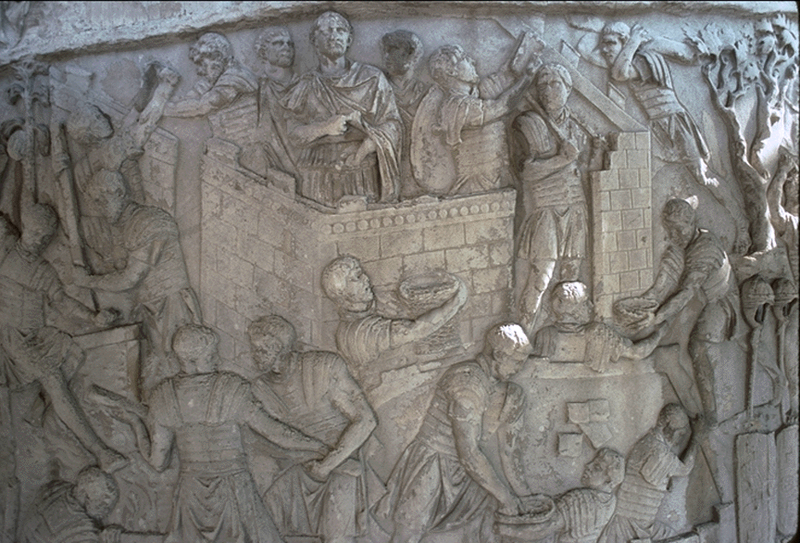
\includegraphics[width=1.1\textwidth]{./graphics/trajan-column}
\caption{Roman soldiers building a fortress, Trajan's Column 113 AD}
\end{figure*}
\end{fullwidth}

Planning is both the organizational process of creating and maintaining a \textit{plan}; and the psychological process of thinking about the activities required to create a desired goal.

\section*{Determining the right sequence of works}

Before any plan is drawn some understanding of the sequence of works
is necessary. Activities can be divided into sequential or parallel. A
sequential activity is one that you cannot start unless a previous activity
has been completed. If the activity of having procured the materials is not
completed, then the works cannot be started. 

\section*{How do I start}

The first thing you need to do before you start is to identify the \textit{goal}.
In many cases this is not that difficult, but you will find out that the goal as
stated is too theoretical and you need to cut it down to smaller objectives.

We will discuss techniques by means of focusing on examples which are smaller.
In my opinion this is where most people fail to plan properly and let events
overtake them. We will assume that shop drawings are available and that materials
are also available and that we will use a Team of Duct erectors.

\subsection*{Measure your target}

Unless you measure something, you cannot control it. If you know that you have to install 600 m$^2$ of ductwork, you may be in a better position to estimate the time
it takes to install it (provided that you have some background information). 


\begin{marginfigure}
The Tower can be represented by a series of squares, which denote an activity. Green is done and white is not done. There is no need to use intermediate colors. they just detract from the visual information.
\vspace{1cm}
%% Color definitions




\floor{Level 47}{0}{0}{0}{0}{2}
\floor{Level 46}{0}{0}{0}{2}{2}
\floor{Level 45}{0}{0}{1}{1}{1}
\floor{Level 44}{0}{0}{1}{1}{1}
\floor{Level 43}{1}{1}{1}{1}{1}
\floor{Level 42}{1}{1}{1}{1}{1}
\floor{Level 41}{0}{1}{1}{0}{1}
\floor{Level 40}{0}{1}{1}{1}{1}
\floor{Level 39}{0}{1}{1}{1}{1}
\floor{Level 38}{0}{1}{1}{1}{1}
\floor{Level 37}{0}{0}{1}{1}{1}
\floor{Level 36}{0}{0}{0}{1}{1}
\floor{Level 35}{0}{0}{0}{1}{1}
\floor{Level 34}{0}{0}{0}{1}{1}
\floor{Level 33}{0}{0}{0}{1}{1}
\floor{Level 32}{0}{0}{0}{1}{1}
\floor{Level 31}{0}{0}{0}{1}{1}
\floor{Level 30}{0}{0}{0}{1}{1}
\floor{Level 29}{1}{1}{1}{1}{1}
\floor{Level 28}{1}{1}{1}{1}{1}
\floor{Level 27}{0}{1}{1}{1}{1}
\floor{Level 26}{0}{1}{1}{1}{1}
\floor{Level 25}{0}{0}{1}{1}{1}
\floor{Level 24}{0}{0}{1}{1}{1}
\floor{Level 23}{0}{0}{1}{1}{1}
\floor{Level 22}{0}{0}{1}{1}{1}
\floor{Level 21}{0}{0}{1}{1}{1}
\floor{Level 20}{0}{0}{1}{1}{1}
\floor{Level 19}{0}{0}{1}{1}{1}
\floor{Level 18}{0}{0}{1}{1}{1}
\floor{Level 17}{0}{0}{1}{1}{1}
\floor{Level 16}{0}{0}{1}{1}{1}
\floor{Level 15}{0}{1}{1}{1}{1}
\floor{Level 14}{0}{1}{1}{1}{1}
\floor{Level 12}{0}{1}{1}{1}{1}
\floor{Level 11}{0}{1}{1}{1}{1}
\floor{Level 10}{1}{1}{1}{1}{1}
\floor{Level 09}{1}{1}{1}{1}{1}
\floor{Level 08}{1}{1}{1}{1}{1}




%
%\begin{tikzpicture}[scale=0.8]
%\draw node [anchor=south east]{Level 08};
%\draw (0,0) rectangle (0.5,0.5);
%\draw  [fill=green] (0.6,0.0) rectangle (1.1,0.5) ;
%\draw [fill=green] (0.6+0.6,0.0) rectangle (1.7,0.5) ;
%\draw[fill=green]  (3*0.6,0.0) rectangle (2.3,0.5) ;
%\draw[fill=green]  (4*0.6,0.0) rectangle (2.9,0.5) ;
%\node at (4,0.1) {Apart. 90\%};
%\end{tikzpicture}
%\def\addlegend#1#2{% color label
%  \begin{tikzpicture}[scale=0.8]
%   \draw[fill=#1] (0,0) rectangle (0.5,0.5);
%   \draw node [anchor=south east]{#2};
%   \end{tikzpicture}\vspace{2pt}}
%\addlegend{green}{lights}
\caption{Rotana Tower Progress, each square represents one separate activity}
\end{marginfigure}


When you first start with the plan, a visual representation of the
areas and work you will be working on can be invaluable. For example
a layout of the area with some coloring can help you identify better
to visualize the problem. At this point if the area is available, you
should visit the area and get a feeling of the problems that you may 
encounter. Once you have a good idea of what you want to achieve, you need to translate
it into something more definable. For ductwork we would normally divide
the work as shown in \ref{ductplan}. For most MEP activities is almost
a rule that unless you put a Team to start by installing supports, it is 
almost certain that manhours will be lost later on. By starting supports early
you ensure that the charge-hand who is marking the support locations is
scouting the area and ensuring that there are no impediments. In very rare
occassions that this is not necessary, such as ductwork in plantrooms.

\pagebreak
\gdef\ascale{0.65}
\begin{minipage}{4cm}
\small
\floor{Level 47}{0}{0}{0}{0}{2}
\floor{Level 46}{0}{0}{0}{2}{2}
\floor{Level 45}{0}{0}{1}{1}{1}
\floor{Level 44}{0}{0}{1}{1}{1}
\floor{Level 43}{1}{1}{1}{1}{1}
\floor{Level 42}{1}{1}{1}{1}{1}
\floor{Level 41}{0}{1}{1}{0}{1}
\floor{Level 40}{0}{1}{1}{1}{1}
\floor{Level 39}{0}{1}{1}{1}{1}
\floor{Level 38}{0}{1}{1}{1}{1}
\floor{Level 37}{0}{0}{1}{1}{1}
\floor{Level 36}{0}{0}{0}{1}{1}
\floor{Level 35}{0}{0}{0}{1}{1}
\floor{Level 34}{0}{0}{0}{1}{1}
\floor{Level 33}{0}{0}{0}{1}{1}
\floor{Level 32}{0}{0}{0}{1}{1}
\floor{Level 31}{0}{0}{0}{1}{1}
\floor{Level 30}{0}{0}{0}{1}{1}
\floor{Level 29}{1}{1}{1}{1}{1}
\floor{Level 28}{1}{1}{1}{1}{1}
\floor{Level 27}{0}{1}{1}{1}{1}
\floor{Level 26}{0}{1}{1}{1}{1}
\floor{Level 25}{0}{0}{1}{1}{1}
\floor{Level 24}{0}{0}{1}{1}{1}
\floor{Level 23}{0}{0}{1}{1}{1}
\floor{Level 22}{0}{0}{1}{1}{1}
\floor{Level 21}{0}{0}{1}{1}{1}
\floor{Level 20}{0}{0}{1}{1}{1}
\floor{Level 19}{0}{0}{1}{1}{1}
\floor{Level 18}{0}{0}{1}{1}{1}
\floor{Level 17}{0}{0}{1}{1}{1}
\floor{Level 16}{0}{0}{1}{1}{1}
\floor{Level 15}{0}{1}{1}{1}{1}
\floor{Level 14}{0}{1}{1}{1}{1}
\floor{Level 12}{0}{1}{1}{1}{1}
\floor{Level 11}{0}{1}{1}{1}{1}
\floor{Level 10}{1}{1}{1}{1}{1}
\floor{Level 09}{1}{1}{1}{1}{1}
\floor{Level 08}{1}{1}{1}{1}{1}
\end{minipage}
\hspace{1em}
\begin{minipage}{4cm}
\small
\floor{Level 47}{0}{0}{0}{0}{2}
\floor{Level 46}{0}{0}{0}{2}{2}
\floor{Level 45}{0}{0}{1}{1}{1}
\floor{Level 44}{0}{0}{1}{1}{1}
\floor{Level 43}{1}{1}{1}{1}{1}
\floor{Level 42}{1}{1}{1}{1}{1}
\floor{Level 41}{0}{1}{1}{0}{1}
\floor{Level 40}{0}{1}{1}{1}{1}
\floor{Level 39}{0}{1}{1}{1}{1}
\floor{Level 38}{0}{1}{1}{1}{1}
\floor{Level 37}{0}{0}{1}{1}{1}
\floor{Level 36}{0}{0}{0}{1}{1}
\floor{Level 35}{0}{0}{0}{1}{1}
\floor{Level 34}{0}{0}{0}{1}{1}
\floor{Level 33}{0}{0}{0}{1}{1}
\floor{Level 32}{0}{0}{0}{1}{1}
\floor{Level 31}{0}{0}{0}{1}{1}
\floor{Level 30}{0}{0}{0}{1}{1}
\floor{Level 29}{1}{1}{1}{1}{1}
\floor{Level 28}{1}{1}{1}{1}{1}
\floor{Level 27}{0}{1}{1}{1}{1}
\floor{Level 26}{0}{1}{1}{1}{1}
\floor{Level 25}{0}{0}{1}{1}{1}
\floor{Level 24}{0}{0}{1}{1}{1}
\floor{Level 23}{0}{0}{1}{1}{1}
\floor{Level 22}{0}{0}{1}{1}{1}
\floor{Level 21}{0}{0}{1}{1}{1}
\floor{Level 20}{0}{0}{1}{1}{1}
\floor{Level 19}{0}{0}{1}{1}{1}
\floor{Level 18}{0}{0}{1}{1}{1}
\floor{Level 17}{0}{0}{1}{1}{1}
\floor{Level 16}{0}{0}{1}{1}{1}
\floor{Level 15}{0}{1}{1}{1}{1}
\floor{Level 14}{0}{1}{1}{1}{1}
\floor{Level 12}{0}{1}{1}{1}{1}
\floor{Level 11}{0}{1}{1}{1}{1}
\floor{Level 10}{1}{1}{1}{1}{1}
\floor{Level 09}{1}{1}{1}{1}{1}
\floor{Level 08}{1}{1}{1}{1}{1}
\end{minipage}
\hspace{0.8cm}
\begin{minipage}{4cm}
\small
\floor{Level 47}{0}{0}{0}{0}{2}
\floor{Level 46}{0}{0}{0}{2}{2}
\floor{Level 45}{0}{0}{1}{1}{1}
\floor{Level 44}{0}{0}{1}{1}{1}
\floor{Level 43}{1}{1}{1}{1}{1}
\floor{Level 42}{1}{1}{1}{1}{1}
\floor{Level 41}{0}{1}{1}{0}{1}
\floor{Level 40}{0}{1}{1}{1}{1}
\floor{Level 39}{0}{1}{1}{1}{1}
\floor{Level 38}{0}{1}{1}{1}{1}
\floor{Level 37}{0}{0}{1}{1}{1}
\floor{Level 36}{0}{0}{0}{1}{1}
\floor{Level 35}{0}{0}{0}{1}{1}
\floor{Level 34}{0}{0}{0}{1}{1}
\floor{Level 33}{0}{0}{0}{1}{1}
\floor{Level 32}{0}{0}{0}{1}{1}
\floor{Level 31}{0}{0}{0}{1}{1}
\floor{Level 30}{0}{0}{0}{1}{1}
\floor{Level 29}{1}{1}{1}{1}{1}
\floor{Level 28}{1}{1}{1}{1}{1}
\floor{Level 27}{0}{1}{1}{1}{1}
\floor{Level 26}{0}{1}{1}{1}{1}
\floor{Level 25}{0}{0}{1}{1}{1}
\floor{Level 24}{0}{0}{1}{1}{1}
\floor{Level 23}{0}{0}{1}{1}{1}
\floor{Level 22}{0}{0}{1}{1}{1}
\floor{Level 21}{0}{0}{1}{1}{1}
\floor{Level 20}{0}{0}{1}{1}{1}
\floor{Level 19}{0}{0}{1}{1}{1}
\floor{Level 18}{0}{0}{1}{1}{1}
\floor{Level 17}{0}{0}{1}{1}{1}
\floor{Level 16}{0}{0}{1}{1}{1}
\floor{Level 15}{0}{1}{1}{1}{1}
\floor{Level 14}{0}{1}{1}{1}{1}
\floor{Level 12}{0}{1}{1}{1}{1}
\floor{Level 11}{0}{1}{1}{1}{1}
\floor{Level 10}{1}{1}{1}{1}{1}
\floor{Level 09}{1}{1}{1}{1}{1}
\floor{Level 08}{1}{1}{1}{1}{1}
\end{minipage}

\pagebreak
\def\don#1{\cellcolor[gray]{0.9}#1}  %{0.9}
\setcounter{inc}{0} % reset counter
\begin{table}[htbp]
\vspace{0.8cm}
\small
\begin{tabular}{|l|p{3.9cm}|l|l|l|l|l|l|l|l|}
\hline
item  &Description  &Qty   &Week 1 &Week 2 &Week 3 &Week 4 &Week 5 &Week 6 &Total\\
\hline
\inc     &supports &400 &\don{100} &\don{100} &\don{100} &\don{100} & & &\\
\inc     &ductwork (insulated) &1200 &\don{200} &\don{200} &\don{200} &\don{200} &\don{200} &\don{200} &\\
\inc     &ductwork (uninsulated) & 600 & & & & & & &\\
\inc     &vol. dampers & & & & & & & &\\
\inc     &fire dampers & & & & & & & &\\
\inc     &flexibles & & & & & & & &\\
\inc     &WIR   & & & & & & & &\\      
\hline
\end{tabular}
\caption{Example of 6 week look-ahead program for installation of ductwork.}
\label{ductplan}
\end{table}

\setcounter{inc}{0} % reset counter
\begin{table}[htbp]
\vspace{0.8cm}
\small
\begin{tabular}{|l|p{3.9cm}|l|l|l|l|l|l|l|l|}
\hline
item  &Description  &qty   &unit & manhours &$f_1$ &$f_2$ &$f_3$ &$f_4$ &Total\\
\hline
\inc     &supports &400 &each & & & & & &\\
\inc     &ductwork (insulated) &1200 &m$^2$ & & & & & &\\
\inc     &ductwork (uninsulated) & 600 &m$^2$ & & & & & &\\
\inc     &vol. dampers &80 &each & & & & & &\\
\inc     &fire dampers &20 &each & & & & & &\\
\inc     &flexibles &60 &each & & & & & &\\
\inc     &WIR   &5 &each & & & & & &\\      
\hline
\end{tabular}
\caption{Example of 6 week look-ahead program for installation of ductwork.}
\label{ductplan}
\end{table}


The factors $f_1, f_2, f_3, f_4$ are a series of factors that ca be used to
adjust your estimate based on your observations of the rate of the works and
the actual conditions that the work is taking place.

$f_1$ = congestion factor.

$f_2$ = weather factor.

$f_3$ = team expertise.

$f_4$ = overtime work.

Of importance is to note that your budget for overtime works will increase
the total manhours that are required to complete the works, as overtime work
in general reduces efficiency of personnel.

The above costs are estimated to be on the low side. Published tables are frequently used to quantify loss of productivity for scheduled overtime [18,19,20,21], overmanning [22,23,24], congestion of trades [23], remobilization [22], and weather [25,26,27].

In this Project the Contractor accelerated completion activities in many areas in order to follow the program. Loss of productivity occurred as a result of overtime due to a number of reasons: fatigue; demotivation; absenteeism; reduction of workpace and congestion, see Figure \ref{fig:congestion}; The factors most commonly cited in the literature are those prepared by the Construction Users' Anti-Inflation Roundatable\sidenote{Construction Users' Anti-Inflation Roundtable, `'Overtime in Construction'', AACE Bulletin, Vol. 15, No. 5, October 1973.}, shown in Figure \ref{fig:overtime}. These impacts have not be taken into account in the above calculations, as the Contractor was aware that overtime, however, inefficient had to be introduced to complete the works by the agreed date. However, not all these costs belong to the Contractor as the Contractor attempted to coomplete Engineer's Instructions and other changes as quick as possible.


\begin{figure}[htbp]
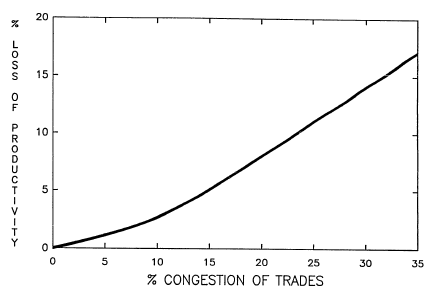
\includegraphics[width=0.9\textwidth]{./graphics/AHU/congestion}
\caption{Impact of overtime on productivity}
\label{fig:overtime}
\end{figure}


\begin{figure}[htbp]
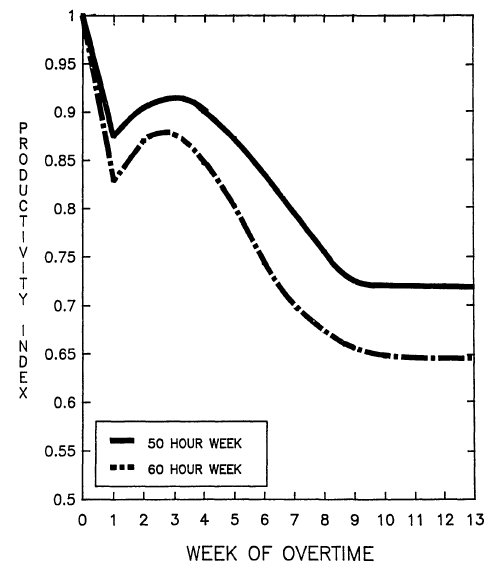
\includegraphics[width=0.8\textwidth]{./graphics/AHU/overtime}
\caption{Impact of overtime on productivity}
\label{fig:congestion}
\end{figure}


The major cause of schedule disruptions and delays all related to lack of information and change orders. Essentially, all causes beyond the Contractor's control

\subsection{Resourcing}

The first step that we discussed so far is how to analyze an activity and
produce a rough estimate of the man-hours required to complete the works.
In the second Table we have added some factors that can assist to determine
productivity; when they are applied they will either increase or decrease
the estimate. 

Once this step has been completed, we need to allocate the necessary resources
to the activity, that is alloacte technicians that are going to carry out the
installation.

My suggestion: when you need to structure a big project, don’t impose a \textit{preferred team} size on people just because it is written in a book. Try to allow self-organization to do its job and let the people (within their real environment) figure out what their optimum is. Do they want to cut a team of seven into two teams of three and four? Sure, why not? Are they merging two teams into one big team of fifteen? Fine, let them see if that works. And be aware that they might want to reconsider things when the environment (or the set of personalities in the team) changes again.

In general though use what it works, but allocate the teams.

A charge-hand can handle up to a 'tent-group' well which should be 5-9 people. We will call these groups, by letters

Ducting Group A

Ducting Group B

Ducting Group C

Ducting Group D

Ducting Group E


\subsection*{The ideal size of a group}

The two-pizza principle can be used to determine an ideal group size. Simply
stated is that you should be able to feed this group with two-pizzas. \sidenote{
Jeff Bezos, has been quoted at \url{http://www.fastcompany.com/magazine/85/bezos_4.html}.} For ductwork
the suggestion is to use 12 people per charge-hand. The rationale behind this
is that this is the maximum size group that a charge-hand can handle well. It
divides into 3 smaller groups of four, which makes installation of heavier
ductwork easier. During third fix activities, it can be split into six pairs
for installation of diffusers.

Some rule of thumbs to allow for ductwork installation that is fully inclusive
of all grilles, diffusers and the like is that you can get a productivity of
approximately 1 m$^2$ per worker. So if you had a full Team able to install 
ductwork for 12 months, out of a 24 month Project to install 100,000 m$^2$ of
ductwork you will need.

\[ n = \frac{100000}{260 \times 12 \times f_1 \times f_2 \times f_3}   \]


If the productivity factors were set to 1 it would require 32 men. Of course the
above is ideal, where one assumes that the workers are working the full day
in ductwork installation, there are are no delays that reduce the productivity.
However, keep this in mind. The other issue is factors relating to the learning
curve and also the fact that work does not always lend it self to a constant
production rate. For smaller ductwork productivity really drops to about less
than half of the above ideal. This also excludes manufacturing of special pieces
tha that necessary, connection of equipment and the like. Those should rather
be measured as individual pieces.

\subsection*{Subdividing the work}

We briefly touched, while discussing productivity factors on the subject
of the \textit{learning curve}. The concept of the learning curve was introduced to the aircraft industry in 1936 when T. P. Wright published an article in the February 1936 Journal of the Aeronautical Science. Wright described a basic theory for obtaining cost estimates based on repetitive production of airplane assemblies. Since then, learning curves (also known as progress functions) have been applied to all types of work from simple tasks to complex jobs like manufacturing a Space Shuttle.

The theory of learning is simple. It is recognized that repetition of the same operation results in less time or effort expended on that operation. For the Wright learning curve, the underlying hypothesis is that the direct labor man-hours necessary to complete a unit of production will decrease by a constant percentage each time the production quantity is doubled. If the rate of improvement is 20\% between doubled quantities, then the learning percent would be 80\% (100-20=80). While the learning curve emphasizes time, it can be easily extended to cost as well.

This simple and now widely accepted principle should be leveraged in your
production planning. For example on high-rise buildings, one should plan
the work vertically, for example one group doing the same activity as they
are going up the Tower See the \ref{towerplan}.

Although, technicians are trained in what they do, the fact that just by moving
around in different areas of the building in unfamiliar surroundings keeps
on affecting productivity. So the rule is to try and plan the works in such
a way that you get the benefit of productivity improvements by using 
repetitive tasks.

\section*{The Gant Chart}

So far we have discussed a number of visual tools and tabular methods to help
assess and plan the works. These are important tools for day to day work and
for work spanning up to six weeks of planning. However, tempting to extend them
to longer periods these will tend to fail as the amount of complexity you adding
prohibits people from understanding them well. In addition if the plan needs
revisions they take took long to modify that one will lose any benefit from
such updates.



%%
% MERWEB TOWER PROGRESS REPORT

\small
\begin{table}[p]
\caption{Merweb Ceiling and Wall Closure Plan}
\begin{tabular}{llllll}
\toprule 
\multicolumn{6}{c}{\bf Merweb Ceiling and Wall Closure}\\
\midrule
~        & Corridor & Pass. lift  & Serv. lift  & Rooms   & Dry walls \\
Level   &            & lobby             &lobby    &    &              \\ 
\midrule
Lvl 43  &             &                &                &             &              \\
Lvl 41  &             &              &         &     &        \\
Lvl 40  & \done     &\done&\done&\done&\done\\
Lvl 39  & \done     &\done&\done&\done&\done\\
Lvl 38  & \done     &\done&\done&\done&\done\\
Lvl 37  & \done     &\done&\done&\done&\done\\
Lvl 36  & \done     &\done&\done&\done&\done\\
Lvl 35  & \done     &\done&\done&\done&\done\\
Lvl 34  & \done     &\done&\done&\done&\done\\
Lvl 33  & \done     &\done&\done&\done&\done\\
Lvl 32  & \done     &\done&\done&\done&\done\\
Lvl 31  & \done     &\done&\done&\done&\done\\
Lvl 30  & \done     &\done&\done&\done&\done\\
Lvl 29  & \done     &\done&\done&\done&\done\\
Lvl 28  & \done     & 27 Jul          &27 Jul         &27 Jul        &\done\\
Lvl 27  & 29 Jul    & 29 Jul   &29 Jul         &29 Jul         &\done \\
Lvl 26  & 2 Aug    & 2 Aug  & 2 Aug        &2 Aug         &\done \\
Lvl 25  & 4 Aug    & 4 Aug  & 4 Aug        &4 Aug         &\done \\
Lvl 24  & 7 Aug    & 7 Aug  & 7 Aug        &7 Aug         &\done \\
Lvl 23  & 9 Aug    & 9 Aug  & 9 Aug        &9 Aug         & 24 Jul\\
Lvl 22  & 11 Aug   &11 Aug & 11 Aug        &11 Aug         &26 Jul\\
Lvl 21  & 14 Aug   &14 Aug  & 14 Aug        &14 Aug         &28 Jul\\
Lvl 20  & 16 Aug   &16 Aug          &16 Aug         &16 Aug         &30 Jul\\
Lvl 19  & 18 Aug   &18 Aug           &18 Aug         &18 Aug         &1 Aug\\
Lvl 18  & 21 Aug   &21 Aug & 21 Aug                  &21 Aug         &3 Aug\\
Lvl 17  & 23 Aug   &23 Aug  &23 Aug         &23 Aug         &5 Aug\\
Lvl 16  & 25 Aug   &25 Aug  &25 Aug         &25 Aug         &7 Aug\\
Lvl 15  & 27 Aug   &27 Aug  &27 Aug         &27 Aug         &9 Aug\\
Lvl 14  & 30 Aug   &30 Aug  &30 Aug         &30 Aug         &11 Aug\\
Lvl 13  & 1 Sep     &1 Sep  &1 Sep         &1 Sep         &13 Aug\\
Lvl 12  & 4 Sep     &4 Sep  & 4 Sep        &4 Sep         &15 Aug\\
Lvl 11  & 6 Sep     &6 Sep  & 6 Sep        &6 Sep         &17 Aug\\
Lvl 10  & 8 Sep     &8 Sep  & 8 Sep        &8 Sep         &19 Aug\\
Lvl 09  & 10 Sep   &10 Sep  & 11 Sep        &11 Sep         &21 Aug\\
Lvl 08  & 12 Sep   &12 Sep  & 13 Sep        &13 Sep         &23 Aug\\
Lvl 07  & 15 Sep   &15 Sep  & 15 Sep        &15 Sep         &25 Aug\\
\bottomrule
\end{tabular}
\normalsize
\label{towerplan}
\end{table}
\normalsize

A Gantt chart is a type of bar chart that illustrates a project schedule. Gantt charts illustrate the start and finish dates of the terminal elements and summary elements of a project. Terminal elements and summary elements comprise the work breakdown structure of the project. Some Gantt charts also show the dependency (i.e., precedence network) relationships between activities. Gantt charts can be used to show current schedule status using percent-complete shadings and a vertical "TODAY" line as shown here.

Although now regarded as a common charting technique, Gantt charts were considered revolutionary when they were introduced[citation needed]. In recognition of Henry Gantt's contributions, the Henry Laurence Gantt Medal is awarded for distinguished achievement in management and in community service. 

\begin{marginfigure}
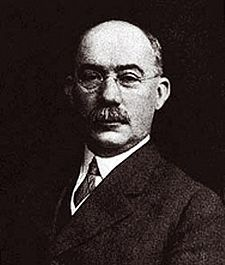
\includegraphics[width=\textwidth]{./graphics/henry-gantt}
\caption{Henry Laurence Gantt, A.B., M.E. (1861 - 23 November 1919) was an American mechanical engineer and management consultant who is most famous for developing the Gantt chart in the 1910s.
These Gantt charts were employed on major infrastructure projects including the Hoover Dam and Interstate highway system and continue to be an important tool in project management.}
\end{marginfigure}


These charts who are produced using Primavera by the Planning Department is
virtually our only tool that communicates the MEP sequence of works to the
rest of the Construction Team. None of the other methods that we have 
discussed handles this intercommunication. During construction though
experienced Construction Managers would normally revert to simpler tabular
or visual methods.

A simple gantt chart (more of a bar chart) can be used to define longer period
activities, that can establish targets. This does not show interdependencies
of activities and for which a more complicated version should be prepared by
the Project Planner. It is important also to bear in mind that if the works 
are delayed for reasons other than owr own (i.e., for example by late information
or by changes) unless there is a good document illustrating these delays it is
extremely difficult to justify the delays.


\begin{fullwidth}
\begin{figure*}[htbp]
\newcommand{\gbar}[3]{\ganttbar[crosshatch, color=orange]{#1}{#2}{#3}}

\definecolor{lightgray}{rgb}{0.7,0.7,0.7}
%% #1 11 rows deep
%% #2 24 cells wide

%% Define short-cuts for months
%%


\def\gantscale#1{}

\newcounter{acount}
\setcounter{acount}{0}
\stepcounter{acount}
\addtocounter{acount}{10}



%\ifnum\theacount>10 number is greater than ten \else number is less than ten\fi


%% Define the months just in case they have not been set
%% before. This needs to be internationalized.
\def\mon#1{\ifcase#1\or%
  Jan\or Feb\or Mar\or Apr\or May\or Jun\or%
  Jul\or Aug\or Sept\or Oct\or Nov\or Dec\else Error 
\fi}


%% a helper macro to add a comma and a space to make the
%% code later on a bit more cleaner

\def\addcomma{, }

%% We define a new counter for looping through the months
%% in order to create the calendar on top
%% this will need to be expanded later 
%\newcounter{monthcount}
%\setcounter{monthcount}{1}
%\whiledo{\value{monthcount}<12}
%  {%
%   \mon{\themonthcount}%
   % adds comma except last one
 %  \ifnum\themonthcount<11 \addcomma\else\relax\fi %
   
  % \stepcounter{monthcount}% 
  %}


%% prints date
%\mon{\numexpr 1+3\relax} \intcalcAdd{\number\year}{1} \relax

%% Global setup
%% 

\xdef\monthstoplot{40}
\xdef\linesdeep{9}

%% Chart drawn in the margins
%% This is the main routine for the chart

%% We define a scale
%
\def\ganttscale#1{#1}



\begin{gantt}[xunitlength=\ganttscale{0.25cm},  fontsize=\footnotesize, drawledgerline=false]{\linesdeep}{\monthstoplot}

%% Define the title of the chart
%%
%% 
\newcommand\GanttTitle[1]{
\ganttitle
    \titleelement{\textsc{#1}}{\monthstoplot}
\endganttitle
}


\GanttTitle{ECU and Black Steel Installation - All Towers}

\begin{ganttitle}
%% We define a new counter for looping through the months
%% in order to create the calendar on top
%% this will need to be expanded later 
\newcounter{monthcount}
\setcounter{monthcount}{1}
\whiledo{\value{monthcount}<11}
  {%
   \mon{\themonthcount}%
   % adds comma except last one
   %\ifnum\themonthcount<11 \addcomma\else\relax\fi %
   \titleelement{\mon{\themonthcount}}{4}
   \stepcounter{monthcount}% 
  }
 
\end{ganttitle}

%% We now loop to typeset the week labels
%% this needs to become more sophisticated
%% as some months do not have 4 weeks
\begin{ganttitle}
   \newcounter{weekcount}
   \setcounter{weekcount}{1}
   \whiledo{\value{weekcount}<11}
  {%
   \mon{\theweekcount}%
   \numtitle{1}{1}{4}{1}
   \stepcounter{weekcount}% 
  }      
\end{ganttitle}
 
%% We define some new colors
\definecolor{red}{rgb}{1,0,0}
% activities are plotted here
\xdef\prop{crosshatch, color=orange}

\ganttbar[\prop]{Rotana }{0}{14}
\ganttbar[crosshatch, color=gray]{Rotana - commissioning}{15}{6}


\ganttbar[crosshatch, color=DarkGreen]{Shangrila}{4}{14}
\ganttbar[crosshatch, color=gray]{Shangrila - commissioning}{19}{6}



\ganttbar[crosshatch, color=DarkGreen]{Merweb}{18}{6}
\ganttbar[crosshatch, color=Gray]{Merweb - commissioning}{24}{3}

\end{gantt}

\caption{All three Towers ECU and black steel installation and commissioning program. Planning provides a safety factor for all Towers for more than two months. We have also allowed for a longer than normal commissioning period in case we are faced with unforseen problems during commissioning.}
\label{plan}
\end{figure*}

\end{fullwidth}



%   
%\section{The gantt package}
%
%In the following you will find a short description of environments and commands: 
%
%The gantt environment draws the canvas of a gantt figure (realized as tikzpicture)
%The usage is |begin{gantt}[...]{no of Tasks to plot}{no of time slots}|
%The optional argument |[...]| can be filled in a |key=value| syntax, using one or more of the following keys:
%
%\begin{description}
%\item [xunitlength]  length of one time slot (default: 1 cm)
%\item [fontsize] fontsize of labels (default: |\normalsize|)
%\item [titlefontsize] fontsize of title section (default: |\small|)
%\item [drawledgerline] Switch to enable/disable the drawing of horizontal ledger lines (default value: false)
%\item [ganttitle] is the environment for drawing the title section
%\item [titleelement] draws one element of the title
%usage: |\titleelement{label}{length}}|
%\end{description}
%
%
%
%
%The \cmd{numtitle} draws a numbered sequence of title elements:
%usage: 
%
%\begin{teX}
%\numtitle{start number}{increment}{end number}{length of each title element}
%\end{teX}
%
%\cmd{ganttbar} draws a single, unconnected bar for representing a task
%usage: 
%
%\begin{teX}
%\ganttbar[pattern]{label}{start}{length}
%\end{teX}
%
%where the optional pattern argument is a tikz pattern, nice patterns for tasks are: 
%north west lines (default), north east lines, crosshatch, crosshatch dots, grid, ...
%
%
%\begin{verbatim}
%\cmd{ganttcon} draws an arrow between to bars with specified coordinates
%usage: \ganttbar{startx}{starty}{endx}{endy}
%
%\ganttbarcon draws a single bar \textit{and} connects the bar with the previous bar for consecutive tasks
%usage: 
%
%\begin{teX}
%\ganttbar[pattern]{label}{start}{length}
%\end{teX}
%
%where the optional pattern argument is a tikz pattern, nice patterns for tasks are: north west lines (default), north east lines, crosshatch, crosshatch dots, grid.
%
%\ganttgroup draws a bar to group tasks
%usage: \ganttgroup{label}{start}{length}
%
%\end{verbatim}
%\section{Physical completion}

%\label{g:test}
%
%\numberLineAt{10}
%\begin{teX}
%\def\mon#1{\ifcase#1\or%
%  Jan\or Feb\or Mar\or Apr\or May\or Jun\or%
%  Jul\or Aug\or Sept\or Oct\or Nov\or Dec\else Error 
%\fi}
%\end{teX}











%These are notes for the gantt chart


\section*{Responsibilities}

Planning spans across all lines of management. Table indicates the type of plans
required and who is responsible to produce them.

\begin{tabular}{lllll}
\toprule
item  &Description            &Prepare   &Check &Approve \\
\midrule
1 &Project Plan               &Planner   &PMs   &Pro. Director\\
2 &6-week look aheads         &Section eng. &PM  &--\\ 
3 &Graphical monitoring plans &Section Eng. &PM  &--\\
4 &Drawings Planning          &CAD Manager  &DM  &PD\\
5 &Materials Planning         &MCD Manager  &PM  &PD\\
6 &Mobilization/demobilization &Planner     &HR  &PD\\
7 &Documentation Plan         &Planner      &DM  &PD\\
8 &Claims                     &Comm.Manager &    &PD\\
\bottomrule
\end{tabular}


\section*{Delays}

Delays and changes to planning are inevitable. As you will recall one of the main 
purpose for developing plans in the first place is to be able to estimate and predict
the impact of events on the end date of the Project. It is the responsibility of the 
Engineer in charge and the Project Manager to identify these delays and appropriate
action be taken to mitigate them, either by requesting more resources to accelerate
the works - once the constraints are removed - or by requesting for an extension
of time.


























\chapter{Engineering}

In our line of work \textit{design} is both ill-defined as well as generally poorly
misunderstood and applied. On most Projects the Owner would have appointed a
Consultant who will produce a design and give it out to tender. In many cases
this is incomplete and supplemented with every conceivable type of clause in a
specification to limit claims by the Contractor. On other type of Contracts we
might have design responsibility for the full works. These are called design-build contracts. In either case a substantial amount of engineering needs to be developed
to complete the design, procure the materials, install the works and putting the
plant into operation.



\section*{The Engineering Department}

On Projects that are not design-build an Engineering Department is set-up with
an Engineering Manager. He is normally assisted with Design Engineers. In addition
he is the ultimate responsible person for overseeing the works of the CAD Office.

\section{Design Audit}

At the start of the Project a quick design audit is undertaken to review the
current design by the Engineer and to identify areas of concerns, missing information and opportunities for savings in costs. This should be summarized in a report with
full details. The same document can then progressively be modified to record all
changes and calculations as works progress.

\subsection*{Selection of equipment}

Equipment selections and submittals fall within the work that the Engineering Department undertakes. As these works might take time to implement the Project Director at the early stages of a Project allocate responsibilities to Senior
Engineers to assist. Some equipment might need calculations before they are ordered as for example fans, pumps, cables, electrical boards and similar items.


\section*{Drawings}

The production of drawings should be done in the \textit{fastest} way possible. 
This is important for two reasons:

\begin{enumerate}
\item As at the beginning of the Project, information might be missing, this is
the best time to record delays, before any \textit{concurrent delays} occur. In many instances the Project Managers or Engineer might issue an information schedule, i.e, a time table listing all the missing information and when this will be issued. Unless this is covered with the Clause (14) programme, one should only accept with the reservation that the Contractot has a right to claim for late information. The Commercial Manager for certain would need to respond. Although
late information for sanitary fixings might not delay the Project it may delay the
drawings and the opening required to accommodate floor mounted units and similar items. If the Engineer has issued a set of IFC drawings no further delays without claims would be acceptable.
\item If works start late on site due to late issue of Shop Drawings or unavailabilty of materials due to late issue of information we would need to add
tradesment to accelerate the works and keep up with the programme. It is always easier to add one CAD Operator than to add 100 tradesmen and more cost effective, given the inefficiencies of disruption and crowded work faces.

\end{enumerate}

\section*{How big a team}

Although, this will depend on the quality of the original design, the number of services involved, the nature of the Project and if the Building has areas where
the design is repetitive a good formula to use is the following:

\begin{equation} n = \sum_{n=1}^{n=k}\frac{f_1}{100}\times C + \frac{f_2}{100}\times C +\cdots+\frac{f_k}{100}\times C_k
\end{equation}

The mimimum size Team should never be less than 16 on Projects that are greater
than QR~200~million.



\section*{Co-ordination}


Possibly more than 70\% of all issues that cause work to stop or to move 
inefficiently can be attributed to poor co-ordination. Although the original
designers bear responsibility for primary co-ordination, we bear responsibility
for co-ordinating the services and for raising the alarm when there are problems
with primary co-ordination.
\begin{marginfigure}
\tikz
\node [forbidden sign,line width=1ex,draw=red,fill=white, scale=2.0] {CLASHES};
\end{marginfigure}

\subsection*{Co-ordination sequence}
At the start of a Project co-ordination needs to follow a sequence of works and
although one will need to go through a number of iterations before the drawings
can be finalized the following sequence will work in most typical cases:

\begin{enumerate}
\item If the ceiling voids have large beams, consider locating the fire mains within the
void provided by the beams to conserve space. Fire mains can easily be sleeved
through and is a good solution, especially in car parks.
\item Drainage pipes should be located hard against the nearest beam and sloped as required, consider changing direction if necessary to have drainage pipes run
shorter routes.
\item It is normal where there is drainage pipes to have cold and hot water. Following a similar route for these pipes would ease co-ordination. 

\item Cable trays should be similarly zoned in parallel with walls. Preferably
no other services should run under or over cable trays to enable clearances for 
pulling cables.

\item Ductwork is a special case and if possible should be run at the lowest level
with flexibles \textit{on the side of the ducts}.

\end{enumerate}

\subsection*{Co-ordination in shafts}

\begin{enumerate}
\item Shaft co-ordination should start early and if possible the first type of co-ordination to take place. This is important as any crossover of services
would seriously reduce ceiling void heights.
\item Always consider providing a platform in shafts. Although this might marginally add to costs, it can speed-up construction tremendously and enable easy hoisting of piping through the shafts.
\item Method of accessible shafts, need to be agreed with stakeholders.
\item For typical plumbing shafts on high rise buildings and or hotels and
apartments consider making an early mock-up--not necessarily in situ--to 
optimize the installation and work out small details such as expansion.
\item Allow adequate space behind ducts and pipes for access to install insulation. This is a normally an overlooked aspect.
\end{enumerate}


\subsection*{Co-ordinators}

Each CAD operator has responsibilty to check his work in terms of
completeness and co-ordination.

\subsection*{Common pitfalls}

\begin{enumerate}
\item One service obstructing another, such as a BMS control box installed too near a fan-coil unit, so that it cannot be opened. This is also common with MCC
boards being too big and cannot be accomodated in Plantrooms.

\item Condensate drains on mechanical equipment that have been - missed on drainage drawings. This can be avoided by showing condensate drains and fan-coil
units on a separate layer and importing this layer on both the VAC drawings
as well as the drainage drawings. Similarly for any equipment requiring power supplies etc.

\item Not allowing an adequate clearance both under or over sectional water tanks.
		This is also a common error by Consultants.

\item Very low plinths for AHUs with high static pressures. This can also happen
		when plinths are designed from structural drawings and then waterproofing is about
		50 mm high ending up with plinths that are only 50 mm high. 

\item Not allowing properly for the curvature of cables when entering switchboards
		or for panels to be ordered bottom entry but the cables are top entry. This is a 
		result of poor scheduling and detailing.

\end{enumerate}



\section*{Professional Drawings}

One can easily recognize a professional drawing when he sees one, but it is 
very difficult to explain what makes a drawing professional.
These are some parameters:

\begin{enumerate}
\item All information required to execute the works is shown on the drawings.
\item Details are specific for the Project and are meaningful.
\item Schedules.
\item Cross referencing.
\item Good choice of pens and styles.
\item The drawing has \textit{dimensions}. 
\item The drawings include sections and larger scale details.
\item The drawing is printed at the right scale.
\end{enumerate}















\chapter{Site Works}

\epigraph{In most people’s vocabularies, design means veneer. It’s interior decorating. It’s the fabric of the curtains and the sofa. But to me, nothing could be further from the meaning of design. Design is the fundamental soul of a man-made creation that ends up expressing itself in successive outer layers of the product or service.}{Steve Jobs}

Siteworks encompass the actual construction. Everything we do is immaterial
unless the works on site can be executed.

\section*{Responsibilities}

Any works on site fall under the responsibility of the relevant Section Engineers.
The Project Manager will manage his section\sidenote{A section of the works
is not necessarily defined by area, but it can also be defined by service for example drainage works will normally fall onto one or two section Engineers, whereas another one might be responsible for a Tower.} of the works but ultimately
the owner of a section of the works is the Project or Site Engineer.


\section*{Resource Scheduling}

The Section Engineer is responsible to plan, monitor the execution of the works
and produce daily and weekly reports as required.

\section*{Workflow}

All Section Engineers and as a matter of fact everyone working on the Project
must be familiar with the standards required of the Project by having read the
specification and by having studied the drawings of his section.

On having been allocated a section of the works the Section Engineer needs to
complete the following activities:

\begin{enumerate}
\item \textit{Review Shop Drawings} One needs to take into consideration that
 Shop drawings might not contain the full information required to carry out the works. The Section Engineer must review the drawings carefully, assist if necessary
with comments that will enable further details to be added and that co-ordination
is possible, ceiling heights achievable and shafts workable.

\item Keep a set of drawings for red-marking.
\item Create a Materials Plan.
\item Prepare Material Take-offs.
\item Issue Site Order Releases.
\item Liaise with Main Contractor for Civil works.
\end{enumerate}


In many instances due to Projects peaking at different times, it is quite likely
that an Engineer will be allocated to a Project during a period that the works
are under pressure. This should not really matter, but then it is still the Section
Engineer's responsibility to make sure that the above steps are followed. If he
is replacing someone that has left the Project then if there is a handover report 
one can verify that the information is correct.

\section*{Site Diary}

All Section Engineer's should keep a Site Diary in which to record the day to
day activities of the works. The Site Diary can be invaluable if claims are
lodged and eventually there is arbitration. The minimum information that must
be logged is:

Area and type of works : start date/end date.

Personnel allocation.

Problems encountered.

Key events related to milestones.

In general keep as much information as possible to enable someone - with your
assistance to recreate the events during the construction period.
\begin{marginfigure}
\includegraphics[width=\textwidth]{./graphics/abandoned-materials}
\caption{Abandoned and dirty materials, make for a very unprofessional work place.}
\end{marginfigure}
\section*{Workface Housekeeping}

There is nothing more wasteful than materials and waste lying all over the
place. The section Engineer must set daily procedures and responsibilities
to ensure that all workfaces are clean, even if this entails cleaning
some of the Main Contractor's rubble that was left behind, when they arrived
and made opening that we \textit{forgot} to tell them about. By keeping the
area clean you ensure that not only it is safe to work but waste is
eliminated and productivity improves. Have an adequate supply of clear plastic
bags for the disposal of rubbish (use clear bags to minimize pilferage).


\section*{Protecting the works}
You should ensure that the works are always protected. All piping and ducting should be wrapped in polyethylene when completed and all open ends closed to minimize the amount of debri and dust that can get in. This ensures that
during commissioning less time is spent in cleaning the system. 


\section*{Damage Reports}

However, hard you try at a point you will reach a stage at which some damages
would occur. These are reported properly using a Damages Report format, which
is issued via the Commercial Department as a claim. Be certain that at the
end of the Project you will face the same from other parties. A damaged works
log is to be kept by the QA/QC Department, as well as Document Control.




\section*{Quality}

Although quality assurance and quality control are handled in a dedicated chapter
we have to mention it here. The Section Engineer is resposnible for the quality
of the works in his area. It takes the same effort to complete the works with the right quality as substandard work. In general the following strategy works
well in raising the bar on quality:

\begin{enumerate}
\item Never accept substandard work
\item Prepare a prototype for all works that you are starting for the 
 first time. This will ensure that all stake-holders and technicians understand
the quality of works required.
\item Offer constructive advise to technicians and supervisors during your
Site Walks for work that just does not look right.
\item Snag the works before you  offer them for inspection.
\item Attend the inspections (if not all of them) at least the ones that 
are offered for the first time or that have failed and are offered again for
inspection.
\item Do not offer works for inspection unless you have checked and can verify
that all materials used are as per approved submittals and the installation is as
per approved drawings. Essentially you must make sure that the materials are
correct and the installation is as per the contract, which in most cases is as
per specification and drawings. Investigate any deviations and take remedial
action if necessary.
\end{enumerate}


\begin{marginfigure}
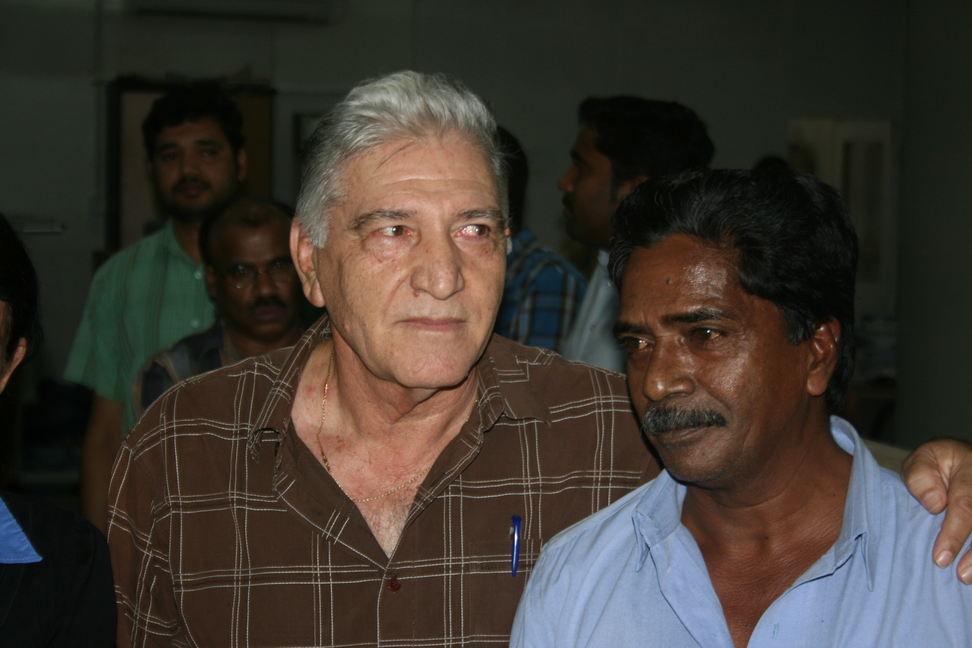
\includegraphics[width=\textwidth]{./graphics/team-spirit}
\caption{Create an environment of openess and co-operation. Quality and targets
are only achieved via a spirit co-operation and Team Work.}
\end{marginfigure}
\subsection*{Quality perception}

Most inspections are \textit{visual} and hence perception psychology plays
an important part. A well lit and \textit{clean} area  with a Team on standby that looks professional, with you having done your homework so that you can answer any question that the
inspector asks will go a long way to a trouble free inspections. With over
30,000 inspections budgeted on larger Projects, if you do not take care of
inspections they are bound to cause delays. 

Other visual items that you will need to take care of is paintwork, supports,
slopes of piping and insulation. 

\begin{marginfigure}
\includegraphics[width=\textwidth]{./graphics/fire-pipes}
\caption{Painted and cleaned piping works and ensuring that nearby pipes run at the same level increase the perception of quality and makes work look professional.}
\end{marginfigure}


\subsection*{Low quality}
If you find that quality is consistently below an acceptable level, make sure 
that you arrange for training for the concerned technicians and or have a prep
talk with everyone. Discuss it with your senior Supervisor and decide what to do.

\section*{Ensure everything will work}

While the daily pressures of work force Engineers to focus on their own section
of works, keep an eye and an enquiry mind to make sure everything works. You 
are the last safety net of both the professional as well as the Contracting Team
to pick up and problems that have not been seen earlier. Ask yourself, will
it work, what happens when something is switched on, can we drain this section
of the works, does it need another valve and so on. You also need to think about
being able to access works for maintenance and also for balancing. So if you have
an access door on a duct taht you cannot open because there is a sprinkler pipe
running across it, you need to take care of it. In general, in this part of the
world, it will cost more to add temporary flushing loops and drains, so ensure
that these have been marked on drawings or take action to request that they are
shown on drawings.




































































\chapter{Quality Assurance and Quality Control}

Quality cannot be accurately defined, but you know it when you see it. On a Site
Quality is the responsibility of everyone and it generally means that you need to
give attention to details.

\section*{The steps to quality}

There are a number of steps that you need to take in order for your work to
be considered quality work and they are really simple.

\begin{enumerate}
\item  Define what you need to do and how to do it. Although the definition part
is simple, it needs to meet the specification, in reality in most cases the specification may be vague. You define the product by making a prototype and by ensuring that it is correct from all angles.

\item Add repeatabiliy

\item Cleanliness

\item Presentation

\end{enumerate}

\section*{The paperwork}

There is a lot of paperwork involved with QA/QC Departments, as a matter of fact perhaps not enough paperwork on a MEP Site as compared to say a manufacturing plant.
\chapter{Communication}

As a rule the medium of communication for Engineers is \textit{drawings}. Engineering is a highly complex field, is information dense and difficult to transmit ideas non-visually. You can have a specification which is six pages long for an example a cooling tower. On a Drawing a simple drawing can describe all that information in a more concise and clear way.

Many other items can be described in traditional documents use in construction:

\begin{figure}
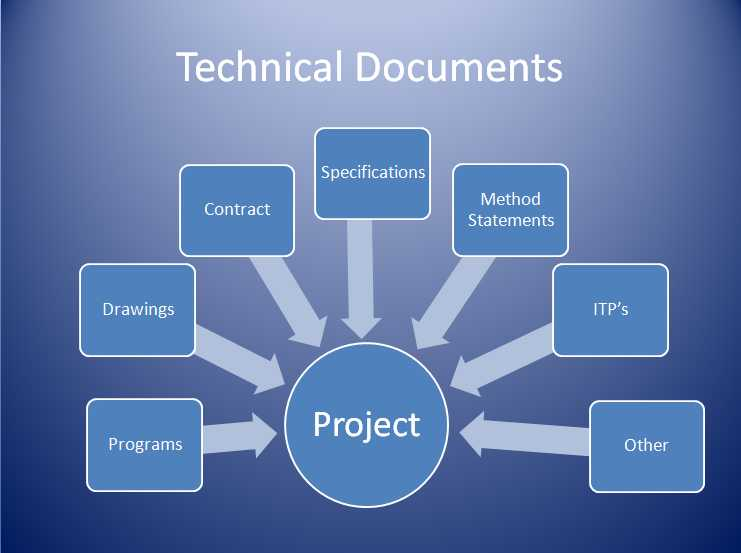
\includegraphics[width=\textwidth]{./graphics/process-02}
\end{figure}

What materials are we going to Supply? This is communicated through technical submittals.

How are we going to install them and test them? This is communicate through ITP's and Method Statements.

When are we going to carry out the work? This is communicated through a Programme of Works.

Who is doing What? This is normally through our organization charts?

Many a better head than this writers have found ways to manage projects along these documents. Although sometimes when misused can cause undue delays, the absence of them can lead to a disastrous Project.

Engineers are not good communicators in general, they work long hours and under pressure making communication more difficult. Try and put as much information on
a drawing as possible. Remember they used to be called plans.


In general we try to commuicate with documents. By utilizing documents rather than verbally communicating requests, actions and the like, documents can flow better. In general use the phone, if you can achieve what you want with the phone-call (such as obtaing the status for something). If the action you request from the person who is next on line will only be completed after a few days commuicate in writing.

\subsection*{Follow-ups}

A message flows better between two people rather than a number of persons. In designing our processes we have kept that in mind. As a rule of thumb if you need to follow-up on a particular action, you need to do it with the person you have send the document to. As an example you have send a request for a purchase. It is no good phoning the Area Manager iff he had approved it or the Financial Department if he has issued the check. You need to follow with the Department head to whom you have addressed the documents. (He might have just finished a meeting with the Financial Manager and a direct call to Accounts, in a way will relieve the MCD Department of his responsibility to expedite)!

\begin{figure}
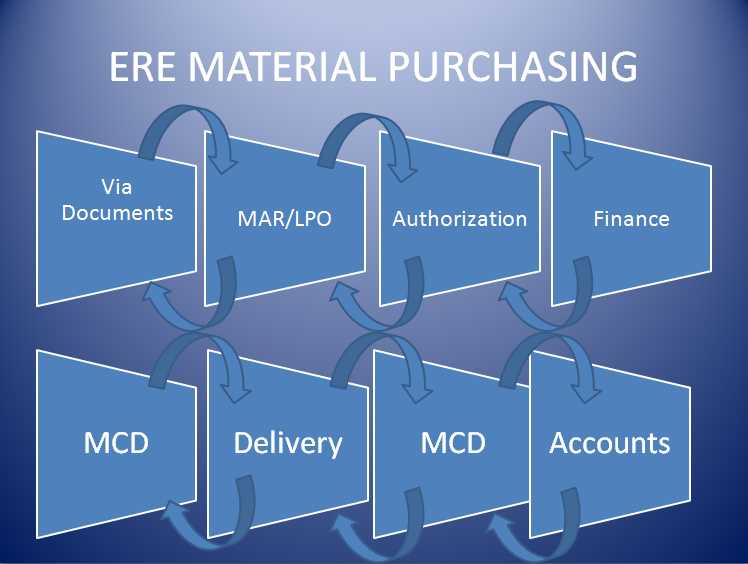
\includegraphics[width=\textwidth]{./graphics/process-01}
\end{figure}

\subsection*{External communications}

Our philosophy is to strive and be professional with our interactions with other Companies. In general we will take a non-confrontational attitude that is pro-active and logical. This does not mean however that we will not stand for our rights.

\subsection*{Documentation}

All documentation with external Companies should be in writing. Either being our own suppiers and sub-contractors or the Client and other members of the professional team. Special care should be taken in approval of variation orders, invoices and other similar issues to our sub-contractors.
\chapter{Contractual}

It is important that all Engineers are aware of the original scope of works. The original scope of works can be found here.

Responsibility for raising the issue of V.O.'s is as follows:

\begin{figure}
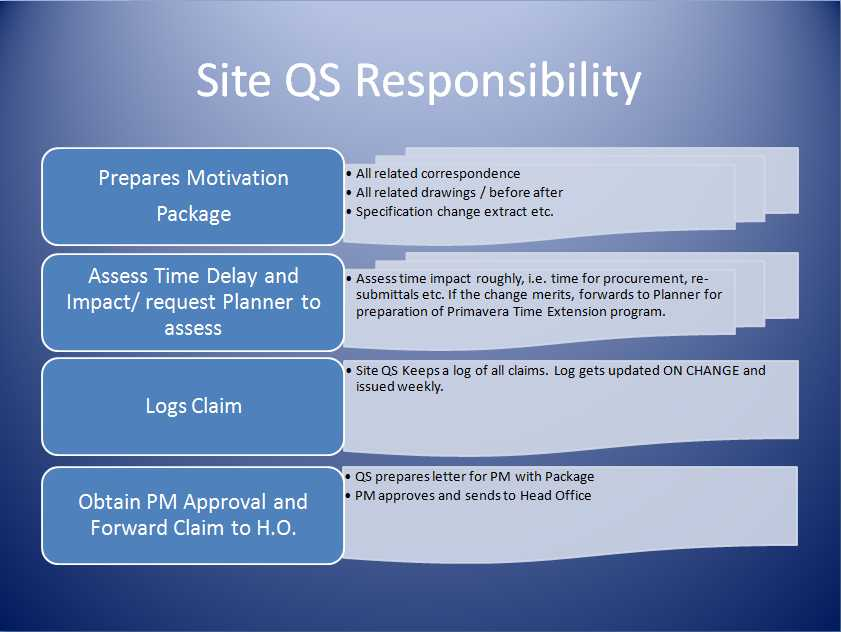
\includegraphics[width=1.3\textwidth]{./graphics/Site-QS-responsibilities}
\end{figure}


It is a very rare occassion that the person originating the change will
issue an instruction and a variation without us asking for it. However,
small this request is, being professional and recording the change will
ensure that in the event that all these minor variations add up, a proper claim
can be lodged.

\section*{Variation Orders}

\subsection*{Awareness}

\begin{tabular}{|l|l|p{2.0cm}|p{2.0cm}|p{2.0cm}|}
\hline
Person &Design Changes&Change via EI, RFI or Letter&Program Changes&Verbal Site Instructions\\\hline
Project Manager    &X&X&X&X\\\hline
Engineering Manager&X& & & \\\hline
Senior Engineers   &X&X& & \\\hline  
Site Engineers     & & & &X\\\hline
Supervisors        & & & &X\\\hline
Planner            & & &X& \\\hline
\end{tabular}  

\section*{Engineers Instructions}

In order to be able to submit a variation as per our contrcat with ADCC and following common practice an Engineers Instruction or otherwise needs to be issued to us. The ONUS is on us to request it.

Copies of Engineers Instructions are sent to H.O. Attention: Mr Fiaz who will then monitor and ensure that it is submitted.

\section*{Site Responsibility}

To issue adequate backgound information for the Variation Order to be submitted. This shold include the `narrative' as well as any other back-up documents.


\section*{Issuing}

All documents to flow through document control. All distribution through document control.

\begin{figure}
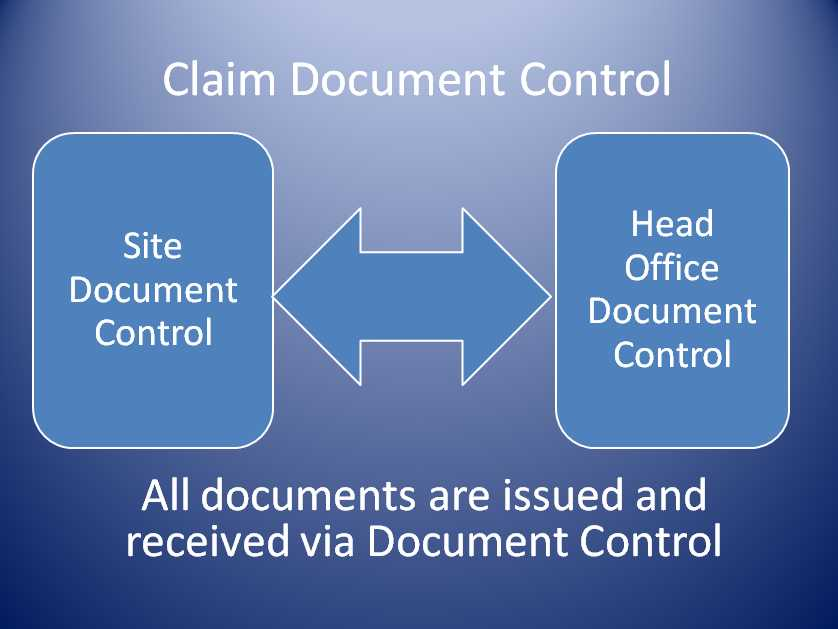
\includegraphics[width=1.3\textwidth]{./graphics/document-control-01}
\end{figure}


\section*{Impact of change orders}

The chart below show the impact of change orders and their distribution. 

\begin{figure}
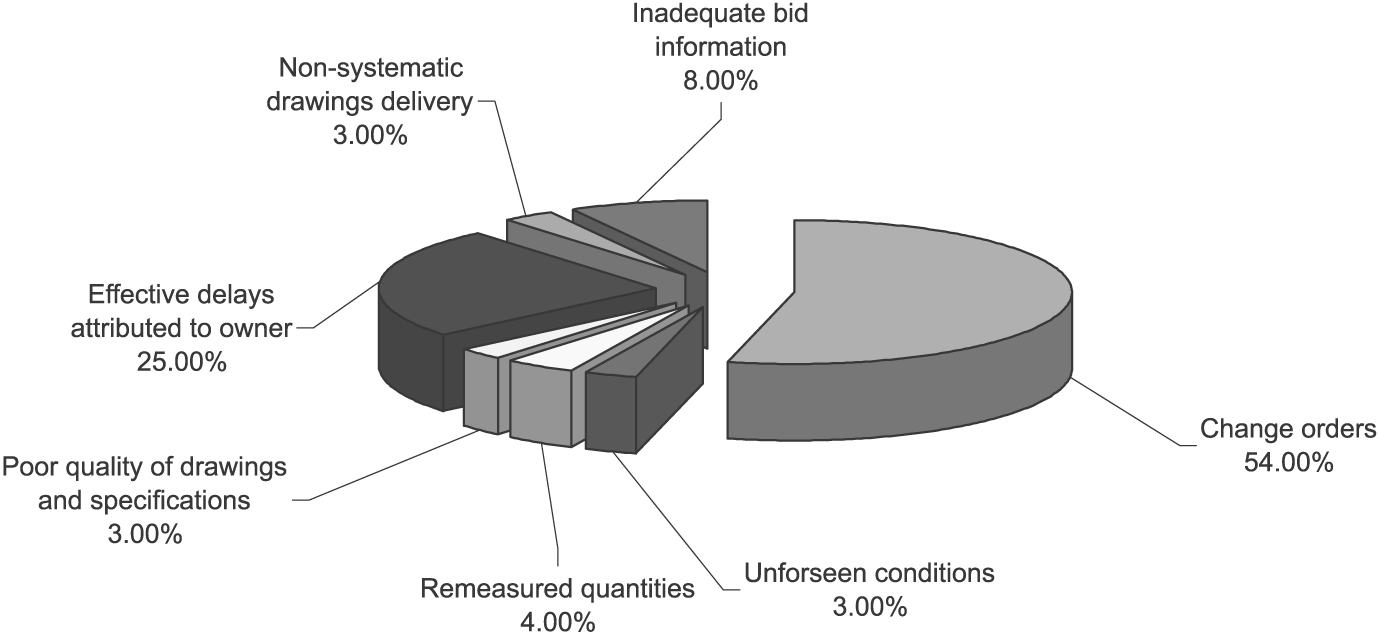
\includegraphics[width=1.3\textwidth]{./graphics/change-orders}
\end{figure}

On Projects where we expect numerous changes we prepare \textit{measle charts}  or
as we call the \textit{chicken pox diagrams}. Like a person afflicted with the
disease your work will be slowed down and the cumulative impact will be much
greater than you think.


\begin{fullwidth}
\begin{figure*}
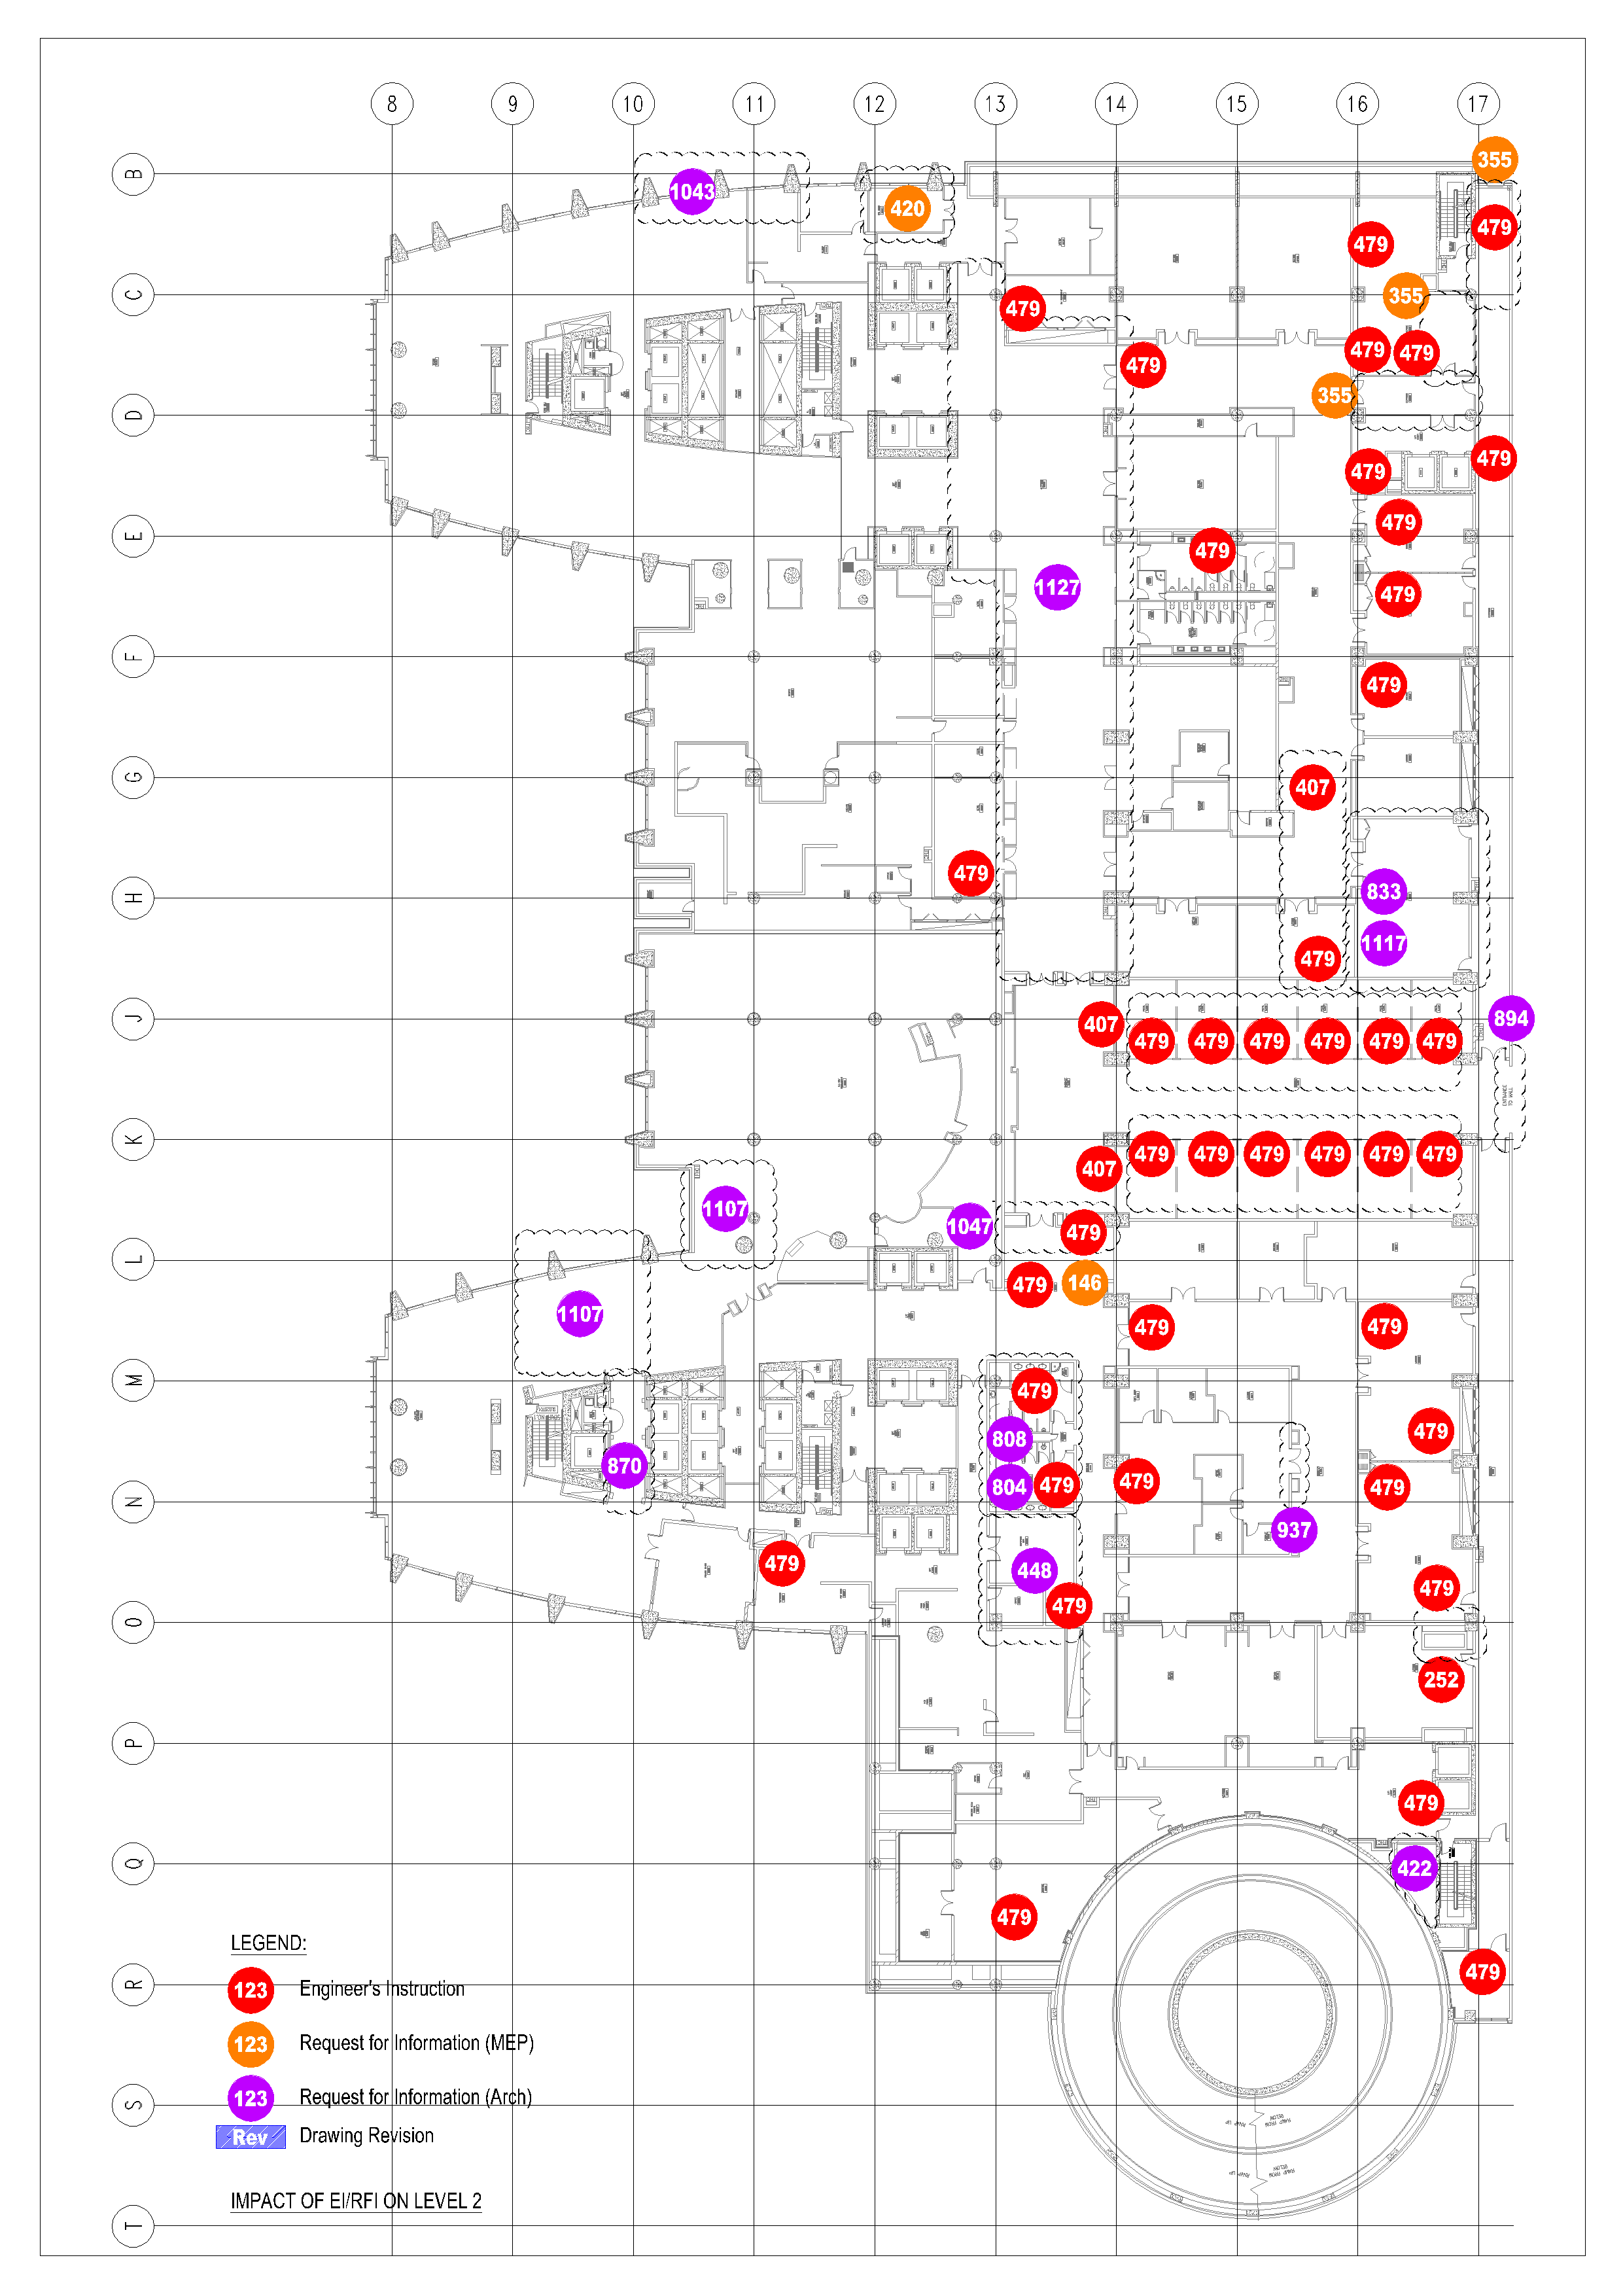
\includegraphics[width=1.1\textwidth]{./graphics/AHU/cpL2}
\caption{Chicken pox diagram showing effect of EIs and major RFIs on a Project.}
\end{figure*}
\end{fullwidth}

\section*{Recording the changes}

Once a Change Order is initiated a number of steps need to be taken
to ensure that contemporaneous records are kept.

The Site QS needs to ensure that a letter is dispatched recording the fact
that the change order will have a time and a cost impact.

The Engineering Manager will need to ensure that the Change Order is reflected
permanently on drawings. The Shop Drawings need to be revised. Please ensure
that revision clouds are included and that the revision text clearly states
the reason for the change.

The Project Manager and Section Engineers will need to assess the impact of
the EI and inform the Commercial Manager of the impact.

The QS will produce weekly and monthly reports as well as record on the
monthly valuations the impact.

\begin{fullwidth}
\begin{table}[htbp]
\vspace{1cm}
\small
\begin{tabular}{l c c c c c c c c c c c c c c c c c c c}
\toprule
~ &Dec & Jan & Feb & Mar & Apr& May & Jun & Jul & Aug & Sep &Oct & Nov &Dec &Jan & Feb  & Total\\
~ &09  & 10  & 10  & 10  & 10 & 10  & 10  & 10  & 10  & 10  &10  & 10   &10 &11&11&11 \\
\midrule
Phase 3a &17 &9 &10 &17 &9 &21 &12 &15 &16 &13 &15 &15 &7 &6&6&187\\
Phase 3b &1   &3 &0 &3 &2 &5 &0 &3 &3 &1 &3 &11 &4 &6&nil&46\\
\midrule
Phase 2a$+$3b &18 &12 &10 &20 &11 &26 &12 &18 &19 &14 &18 &26 &11 &12&16&233\\

\bottomrule
\end{tabular}
\hskip-10cm\caption{Total number of EIs received since the MOU}
\label{tbl:EI}
\end{table}
\end{fullwidth}

\begin{fullwidth}
\begin{table}[htbp]
\vspace{1cm}
\small
\begin{tabular}{l c c c c c c c c c c c c c c c c c c c}
\toprule
~ &Dec & Jan & Feb & Mar & Apr& May & Jun & Jul & Aug & Sep &Oct & Nov  & Dec & Jan & Feb & Total\\
~ &09  & 10  & 10  & 10  & 10 & 10  & 10  & 10  & 10  & 10  &10  & 10   &10 &11 & 11& 11\\
\midrule
Phase 3a &34  & 38  & 63  & 51  & 56 & 50  & 51  & 79  & 32  & 36  &32  & 41   &31&38&17&661 \\
Phase 3b &12 &19 &12 &7 &28 &24 &23 &21 &5 &8 &12 &13 &5&6&7&204\\
\midrule
Phase 2a$+$3b &46 &57 &75 &58 &84 &74 &74 &100 &37 &44 &44 &54 &36&44&24&865\\

\bottomrule
\end{tabular}
\caption{Total number of RFIs issued since the MOU}
\label{tbl:RFI}
\end{table}
\end{fullwidth}


Charts can assist to better visualize problems with Engineer's Instructions
and RFIs.

\chapter{Cumulative Impact of other EIs and RFIs}
\newthought{A growing list of Engineer's Instructions and Requests for Information} followed-up, the signing of the Memorandum of Agreement. The growth of the EIs is shown graphically in Figure~\ref{EIplots}. As at the end of May 2011, there were 300 EIs issued and 1054 RFIs.
Not only the Engineer failed to complete his design by the 15th of December 2009, as agreed with the Contractor and recorded in the Contractor's approved 6.2 Programme of Works, but the Engineer continued with changes well into a year after the planned Completion Date.


\def\monthnames{{"D","J","F","M","A","M","J","J","A","S","O","N","D"}}
\pgfplotsset{width=16cm}

\begin{fullwidth}
\begin{figure*}[htbp]
\begin{tikzpicture}
    \begin{axis}[
        smooth,
        stack plots=y,
        area style,
        enlarge x limits=false,
        ymin=0,ymax=1500,
        xlabel=\textsf{December  2009 to May 2011},
        ylabel=\textsf{Number of Eis and RFIs},
        xtick=data,
        %no need to repeat months more than a year
        xticklabel={\pgfmathparse{\monthnames[Mod(\tick-1,12)]}\pgfmathresult}]
\addplot[color=orange,fill=orange!60] coordinates
		{(0,0) (1,52) (2,103) (3,178) (4,236) (5,320) (6,394)%
                (7,469) (8,569) (9,606) (10,650) (11,695) (12,752)%
                (13,788) (14,833)  (15,881) (16,946) (17,996) (18,1041)
               } 
		\closedcycle;
	\addplot[color=orange,fill=orange] coordinates
		{(0,0) (1,21) (2,32) (3,45) (4,66) (5,78) (6,106)%
                (7,120) (8,138) (9,157) (10,173) (11, 196) (12,223)%
               (13,233) (14,248) (15,262) (16,273) (17,284) (18,299)
               }
		\closedcycle;
    \addlegendentry{\textsf{Requests for Information}}
    \addlegendentry{\textsf{Engineer's Instructions}}
    
   
 
    \end{axis}
\end{tikzpicture}
\caption{Plots showing the growth of Engineer's Instructions and their relationship to Requests for Information, the relationship can be observed clearly. See for example the \textit{bumps} at around April-May 2010.}
\label{EIplots}
\end{figure*}
\end{fullwidth}

No Project, where the Design is incomplete can be completed. It is obvious neither the Owner that could instruct the Engineer to add resources to his Team, nor the Engineer considered the Completion Date to be of \textit{essence}.

The Contractor on its part, accelerated works in sections that were critical for the Owners Direct Contractor to have access, providing this access at the end of June 2010.

% start tikzpicture,define styles
% define a style called activity
\tikzstyle{activity}=[draw,
                      rectangle,
                      rounded corners, 
                      fill=black!5,
                      thick,
                      minimum width=2.9cm,
                      minimum height=2.2cm, 
                      text width=2.5cm
                      ]
\begin{figure*}
\begin{tikzpicture}[mystylei/.style={draw,ellipse,rounded corners, fill=gray!23,thick,minimum
width=3cm,minimum height=1cm, text width=2.5cm, text centered}]


%start to define nodes relative to each other
\newcommand\addblock[2]{\node[activity, node distance=0] (#1) {\textsc{\textbf{#1}}. \textsf{#2}};\def\temp{#1}}

\def\addblockbelow#1#2{\node[activity] (#1) [below=of \temp] {#1. \textsf{#2}};\draw[->] (\temp) -- (#1);
\def\temp{#1}
}

\addblock{1}{Mark EI or RFI implications on drawings}
\addblockbelow{B}{EM to identify implications}
\addblockbelow{C}{Issue Impact form to CM}
\addblockbelow{D}{Obtains approval for revisions. iterates if necessary.}
\addblockbelow{5}{Obtains approval for revisions. iterates if necessary.}


%%\node[activity] (C) [below=of B] {C. Issue Impact form to CM}; 
%\node[activity] (D) [below=of C] {D. Obtains approval for revisions. iterates if necessary.};

%second column with a bit of a distance
\node[activity,node distance=1.3cm] (E) [right=of 1] {E. Commercial Manager, reviews};  
\node[activity,node distance=1.3cm] (F) [right=of B] {F. Impact Forms};
\node[activity,node distance=1.3cm] (G) [right=of C] {G. issue claim}; 

%% Third column      
\node[activity,node distance=1.3cm] (H)  [right=of E] {H. PM reviews}; 
\node[activity, node distance=1.3cm] (J) [right=of D] {J. Cause, narrative};

\node[activity,node distance=1.3cm] (H1) [right=of F] {H1. Plans the works. Issues stop orders if necessary};

%empty node for the gap in column 2 row 3
  
\node[activity,node distance=1.3cm] (K) [right=of G] {K. Issue Impact Form to CM. Photographic records};       
\node[activity,node distance=1.3cm] (H2) [right=of J] {H2. Arranges materials and installation (WIR)}; 



%connect the nodes
%\draw[->] (1) -- (B);
%\draw[->] (B) -- (C);
%\draw[->] (C) -- (D);
\draw[->] (E) -- (F);
\draw[->] (F) -- (G);
\draw[->] (G) -- (J);
\draw[->] (C) to [out=360,in=180] (F);
\draw[->] (D) to [out=360,in=199] (F);
\draw[->] (K) to [out=180,in=360] (F);
\draw[->] (H1)-- (K);
\draw[->] (H) -- (H1);
\draw[->] (K) -- (H2);
%\draw[->] (C) -- (K);

\end{tikzpicture}
\caption{Workflow for Engineers Instructions and RFI works. All Departments get involved when there is a Change Order. Evaluate Change Orders as they occur and keep contemporaneous records. }
\end{figure*}







































\chapter{Handover}

It is important that all Engineers are aware of the original scope of works. The original scope of works can be found here.

Responsibility for raising the issue of V.O.'s is as follows:

\begin{figure}
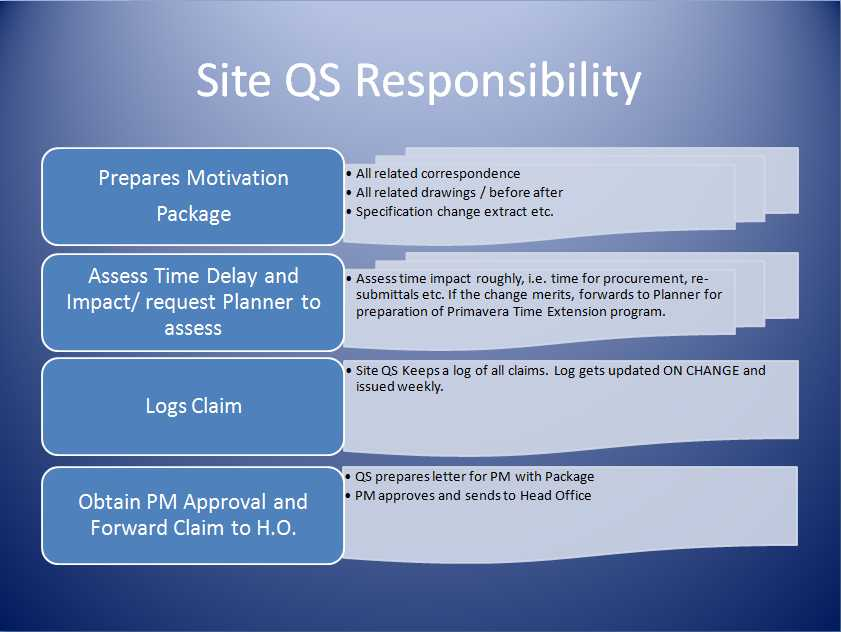
\includegraphics[width=1.3\textwidth]{./graphics/Site-QS-responsibilities}
\end{figure}

\section*{Hand Over Documentation}

The aim of collating all documentation at the end of a Project in order to verify that all parties have inspected and accepted the Installation. These documentation will have to be enclosed in the Operations and Maintenance Manuals.

\section*{As-Build Drawings}

This is the most basic requirements and in an ideal Site they will be produced as an on-going activity, while the Site is operating. Remember that every change on the AS-BUILDS points to lack of good engineering at the beginning of the Project and to an extent lack of planning. Minor changes are understandable to incorporate Site instructions but any large scale operations to update drawings is as a sad story.

\section*{Proof that the Works have been Physically Inspected}

A list of all WIR's properly collated should be summarized.
Contractor's confirmation that the works have been completed.

\section*{Proof of commissioning}


\section*{The Final Touch}

Depending on the specification, the Designers might have even elected to
specify the font and the font-sizes for the manual. The OM manuals will
impact on our brand long after we have left the project. It is important that
they look professional and that they are bound correctly. Drawings and CDs
should be copied properly.











%\chapter{Business edge}

\section*{Introduction}

In order to build a business edge we need to define the business better, decide on the sector we are operating in and build an edge that will differentiate us from our competitors.

\subsection{What are we offering}
Are we selling materials, which we incidentally install? Are we selling services, integrate Suppliers and Subcontractors and execute the works? What is our \textbf{product}?

Our product should be focused well defined and enable us to sell it in a way we differentiate from the opposition.
Our main opposition can be divided into three main groups:

\begin{itemize}
\item Low cost Companies, mostly from India suh as ETA and Voltas. Some of these Companies as for example Voltas, are backed by big groups operating in many sectors. Both ETA and Voltas have relationships with factories in India, giving them an edge on prices. A Project that has accepted an Indian subcontractor is amenable to Indian quality products that are currently unbeatable in prices.
\item International European Firms, such as Thermo 
\item Local Companies, backed by serious money  for example Al-Futeim Group's Carillion. These Companies work both on price as well as their ability to network.
\end{itemize}

\subsection*{Clients}

Clients are mostly Main Contractors, although direct nomination by Owners and Project Manager's is a possibility. Other stake holders in the approval process are Consultant's and Owner representative firms. Very little work so far has been carried out directly with Government Organizations.

\subsection*{Image}

Although one can say the image we want to project is one of professionalism, that is too general. In order to lay out the requirements and needs of the amrket and translate them to a Product one need to rethink the total operations.

\textbf{During project Execution.}\quad
The most important image we need to project is one of \textit{effortless} execution. What I mean with effortless execution, is that we need to execute all the stages of the Project with proactive resolution of issues, meeting of \textit{all} deadlines, from a promise to deliver a document or letter to installation works, to fitting our operations with those of the Main Contractor.

In order to achieve this a number of prerequistes need to be met, which we will analyze a bit later, a simple interpretation of this requirement is the need to stay ahead rather than be behind the Design team or teh Main Contractor's Team. Simply translated add well organized resources at the early stages of the Project.

\texbf{Paper work.}\quad During the life time of the Project, until perhaps the 60\% stage performance is mostly judged on \textit{paper work}. Method Statement for a new Project can be delivered in a well \textit{typeset manner} within the first month of the Project. they are repeated from Project to Project and the reason why the are re-written every time, is that no-body has perfected them to the point that they satisfy a different set of Project Managers. If the sections and the write up is ready, it is quite possible to achieve this and \textit{automate} it. On a large Project, what should be a minor cost translates to a constant hassle that probably is equal to the cost of one Engineer for the duration of the Project. With the right investment in preparing these upfront it is possible to reduce this cost substantially and improve our image. 

\textit{Submittals}\quad
This is normally a horror story. It is not unknown that it can take up to a year to get some materials approved. The problem here starts from getting quotations, getting the supplier approved from everyone involved and then writing up the submittal (normally the supplier will draft it up---which in many instances due to format problems, it gets rejected). 

\textit{Drawings}\quad Here one needs to lift the barriers of quality. Good drawings save money and accelerate the works. The duration for drawing production should be worked out on 3 months for first iteration and a six month window for A status full set of drawings. If there are change orders, resource can be added accordingly at a later stage, plus claiming overheads for the Engineering Team.

``Cats are intended to teach us that not everything in nature has
a function.''

Garrison Keillor (1942–)

\section{Improving Production and Focusing on our Product}

Consider the possibilities. A recent survey of published results by manufacturing
and service companies that have applied constraint management
methods effectively shows:\footnote{Source: Mabin, Victoria J. and Steven J. Balderstone,
The World of the Theory of Constraints:A Review of the International Literature, St. Lucie Press, Boca Raton, FL, 2000.}

\begin{enumerate}
\item A mean reduction in lead times of 70\%

\item A mean reduction in manufacturing cycle times of 65\%

\item A mean improvement in due-date performance of 44\%

\item Mean inventory reductions of 49 percent

\item A mean combined financial improvement (revenue, throughput,
profit) of 76.\%

\end{enumerate}

I am convinced that as applied to the Construction Industry this might even be an understatement. I am also convinced that the actual methodology will have to be improved, but one wonders why this is not happening.

\begin{figure}
\leftskip20pt \rightskip20pt
Peninsula Daily News
(Associated Press), Port Angeles, WA,

Monday, Aug. 2, 1999, p. A5

Delays in spray paint delivery curtail Forest Service harvests

Associated Press

Logging in federal forests is down by as much as 25 percent this year in regions
outside the Northwest because the U.S. Forest Service can’t find enough of the paint
it needs to mark trees for cutting. The agency says that it will try to make up the
logging deficit by next year at the latest.
The paint shortage so far has not had an impact on timber sales in Washington
and Oregon. “We still have paint, but we’re running low — and we have an emergency
order in,” spokesman Rex Holloway said.
Timber sales in the five-state Rocky Mountain region are down between 15 and
25 percent because of the paint shortage, forest officials said. Many of the other nine
regions are in “roughly the same ballpark,” although they could catch up before the
end of the year, said Ann Bartuska, director of forest management for the Forest
Service in Washington, D.C. “People are coping perfectly well,” she added.
Some foresters are marking trees the old fashioned way while they wait for the
paint — using a hatchet to notch the trees, Bartuska said.
The agency on May 15 stopped using, oil-based paint to mark the trees it plans
to cut down, after workers blamed the paint on an increase in miscarriages and other
ailments. But Bartuska said the transition to water-based paint was more difficult
than expected. There was an explosion at a paint factory, procurement delays by the
General Services Administration and delays in getting the forest workers’ union to
approve the new paint.
“Everything that could go wrong has gone wrong,” she said, adding that the Forest
Service is rushing as much paint out to forests as it can.
Timber sales in the Rocky Mountain region — South Dakota, Nebraska, Kansas,
Wyoming and Colorado — will be down between 30 million and 51 million board
feet this year, regional forester Lyle Laverty said, in a letter earlier this month. That
disclosure prompted a letter last week from six senators to Forest Service Chief Make
Dombeck.
``These downfalls are not acceptable,''  the senators from Wyoming, South Dakota
and Colorado wrote.

\copyright 1999, The Associated Press. All rights reserved. Reprinted with permission.

\end{figure}


To know with confidence that a local decision truly advances the goal of
the company (which we assume for most organizations is to
make money), we need to understand how such decisions actually impact
the global financial performance of the organization---if they do at all. What
management needs is a new set of yardsticks that enhances decision making
at all levels. These yardsticks should provide a clear, unequivocal connection
between local decisions and global performance. They should motivate functional
managers to make the right exploitation and subordination decisions
--- the decisions that improve the whole organization’s performance, not just
their own department’s. And these yardsticks must be simple and easily
understood by everyone.







%\input{./manual/blog}


\backmatter
%\bibliography{sample-handout}
%\bibliographystyle{plainnat}
\printindex

\end{document}
Dreyfus competence model
https://en.wikipedia.org/wiki/Dreyfus_model_of_skill_acquisition

























